\chapter{Outras Funções}
\section{Introdução}

\begin{justify}
\quad Nos capítulos anteriores estudamos as funções de 1º e 2º grau, que são funções polinomiais. Uma série de outras funções são utilizadas para modelar problemas de ciência e tecnologia como funções potência com expoente fracionário, racionais, polinomiais com grau maior do que dois, funções modulares e funções com mais de uma sentença.
\end{justify}

\section{Funções potência}

\begin{caixa}
\begin{tdefinicao}
As funções potência têm a forma 

\quad  \( f \left( x \right) = Ax^{m} \), sendo $A \in \mathbb{R}$ e $m \in Q^{+}.$\quad \quad \quad \quad (2.1)

Se  \( m=\frac{a}{b} \)  com \textit{a} e \textit{b} $ \in $  \textbf{\textit{Z}} ,com \textit{b $ \neq $  0}, \textit{f(x)} pode ser escrita como uma raiz:

\quad  \( f \left( x \right) =A\sqrt[b]{x^{a}} \) \quad \quad \quad \quad \quad \quad \quad \quad (2.2)

\quad Na forma da Eq. (2.2), se \textit{b} é par, \textit{f(x)} só é real se o radicando for positivo \qedsymbol{} 
\end{tdefinicao}
\end{caixa}

\begin{texemplo}

Faça o gráfico, determine o domínio e a imagem da função  \( f \left( x \right) =x^{2/3} \)  (ou  \( f \left( x \right) =\sqrt[3]{x^{2}} \) ).

\textbf{Solução}: A função dada é uma função potência, pois o expoente é um número racional. Atribuindo valores para \textit{x,} obtemos os valores de \textit{f(x)} com o uso de uma calculadora. 

\begin{figure}[H]
\begin{Center}
        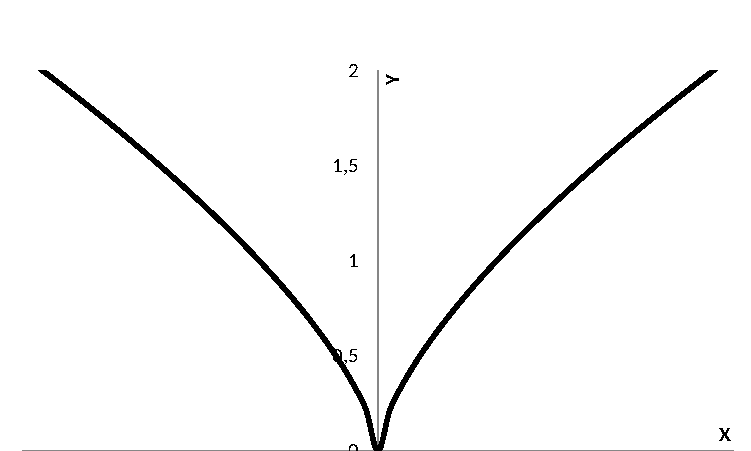
\includegraphics[width=3.65in,height=2.35in]{capitulos/outras_funcoes/media/image2.pdf}
    \end{Center}
\end{figure}
~~

\quad O gráfico desta função potência também pode ser obtido escolhendo valores de \textit{x\textsuperscript{2}} cuja raiz cúbica seja inteira, tais como: \textit{0, 8, 27}. Os respectivos valores de \textit{x} serão: 0,  \( \sqrt[]{8} \) ,  \( \sqrt[]{27} \) ~ . Com os pontos (0,0),( \( \sqrt[]{8} \) ,2) e ( \( \sqrt[]{27} \) ,3) pode-se traçar um bom esboço do gráfico de \textit{f(x)}.

\quad Escrevendo a função como uma raiz:~  \( y=\sqrt[3]{x^{2}} \) .

Pode-se observar que: 

(i) será possível calcular os valores de \textit{y} para qualquer valor de \textit{x}, pois existe raiz cúbica de qualquer número real. Portanto: \textit{Df(x)=$ \{ $  x $ \in \mathbb{R} $  $ \} $ .}

(ii) não existirá \textit{y < 0} pois todos os valores de \textit{x} estão sendo elevados ao quadrado e a raiz cúbica destes será nula ou positiva. Portanto: \textit{I\textsubscript{m}f(x)=$ \{ $ y $ \in \mathbb{R} $   / y $ \geq $  0$ \} $ }\qedsymbol{}
\end{texemplo}
 
\begin{texemplo}
	
Faça o gráfico, determine o domínio e a imagem da função  \( f \left( x \right) =x^{3/2} \).

\textbf{Solução:} A função dada é uma função potência, pois o expoente é um número racional. Atribuindo valores para \textit{x,} obtemos os valores de \textit{f(x)} com o uso de uma calculadora. 

\begin{figure}[H]
	\begin{Center}
		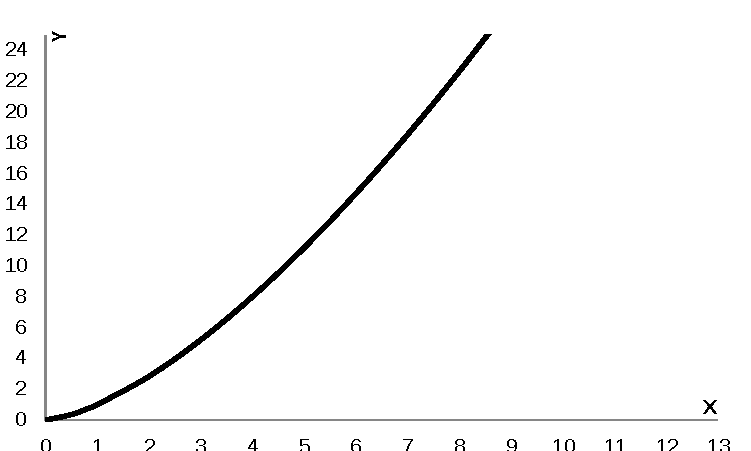
\includegraphics[width=3.59in,height=2.35in]{capitulos/outras_funcoes/media/image3.pdf}
	\end{Center}
\end{figure}

~~

\quad Temos~a opção de escrever a função como uma raiz:   \( y=\sqrt[]{x^{3}} \).

Pode-se observar que: 

\begin{enumerate}
	\item será possível calcular os valores de \textit{y}, apenas para  \textit{x $ \geq $  0}, pois se \textit{x < 0} o radicando será negativo e a raiz quadrada não será real. Portanto: \textit{Df(x)=$ \{ $  x $ \in \mathbb{R} $ / x $ \geq $  0$ \} $ .}

	\item não existirá \textit{y < 0} pois todas as raízes quadradas serão nulas ou positivas. Portanto: \textit{I\textsubscript{m}f(x)=$ \{ $ y $ \in \mathbb{R} $   / y $ \geq $  0$ \} $  }\qedsymbol{} 
\end{enumerate}
\end{texemplo}

\begin{texemplo}
	
Faça o gráfico, determine o domínio e a imagem da função  \( f \left( x \right) =x^{1/3} \) .

\textbf{Solução:} A função dada é uma função potência, pois o expoente é um número racional. Atribuindo valores para \textit{x,} obtemos os valores de \textit{f(x)} com o uso de uma calculadora. 

\begin{figure}[H]
	\begin{Center}
		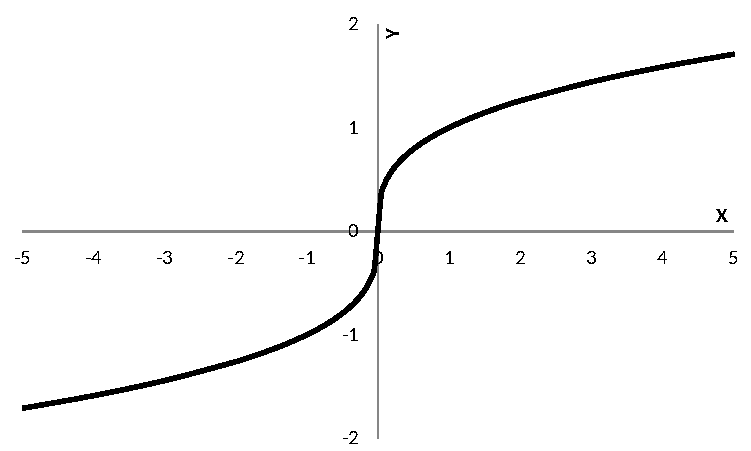
\includegraphics[width=3.6in,height=2.41in]{capitulos/outras_funcoes/media/image4.pdf}
	\end{Center}
\end{figure}

~~

\quad 

Temos~a opção de escrever a função como uma raiz:   \( y=\sqrt[3]{x^{}} \)  e observar que: 

\begin{enumerate}
	\item Como a raiz é cúbica será possível calcular os valores de \textit{y} para qualquer  \textit{x} real. Portanto: \textit{Df(x)=$ \{ $  x $ \in \mathbb{R} $  \textbf{ }$ \} $ .}

	\item \textit{ }O gráfico indica que -$\infty$ < y < + $\infty$\textit{. } Portanto: \textit{I\textsubscript{m}f(x)=$ \{ $ y $ \in \mathbb{R} $  $ \} $  }\qedsymbol{} 
\end{enumerate}
\end{texemplo}

\begin{texemplo}
	
Determine a concavidade das funções potências para \textit{A = 1}~ e~ \textit{0 < m < 1;~ m =1}~~~e  \textit{m > 1}. 

\textbf{Solução:} As figuras abaixo apresentam os gráficos para funções potência com \textit{A = 1}~ e  \textit{m} nos intervalos dados. 

\begin{figure}[H]	
	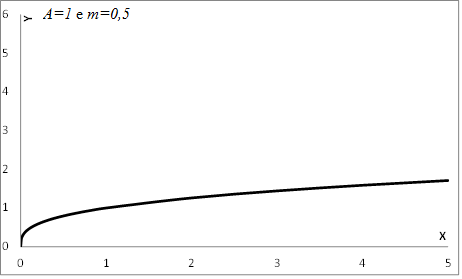
\includegraphics[width=0.45\textwidth]{capitulos/outras_funcoes/media/image5.png} 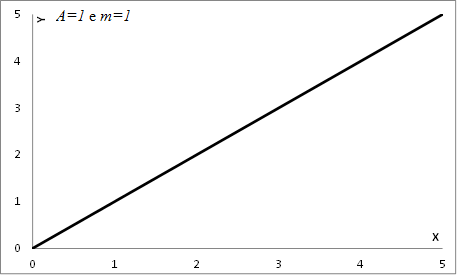
\includegraphics[width=0.45\textwidth]{capitulos/outras_funcoes/media/image6.png}
\end{figure}

\begin{figure}[H]
	\begin{Center}
		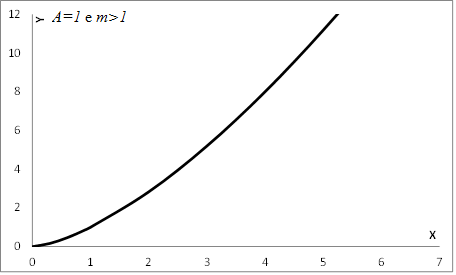
\includegraphics[width=3.3in,height=2.29in]{capitulos/outras_funcoes/media/image7.png}
	\end{Center}
\end{figure}

~~

\begin{enumerate}
	\item Para  \textit{0 < m < 1} : concavidade para baixo.

	\item Para \textit{m = 1}, a função potência é a própria função identidade. Não tem concavidade pois é uma reta.
	
	\item Para \textit{m > 1}~~ : concavidade para cima \qedsymbol{}  
\end{enumerate}
\end{texemplo}

\begin{texemplo}
	
Faça o gráfico, determine o domínio e a imagem da função  \( f \left( x \right) = \left( x+1 \right) ^{1/2} \) .

\textbf{Solução:} Observemos que à base da potência foi acrescentada uma soma ao \textit{x}. O efeito no gráfico é um deslocamento, neste caso para a esquerda, do gráfico da função  \( f \left( x \right) = \left( x \right) ^{1/2} \) .

\begin{figure}[H]
	\begin{Center}
		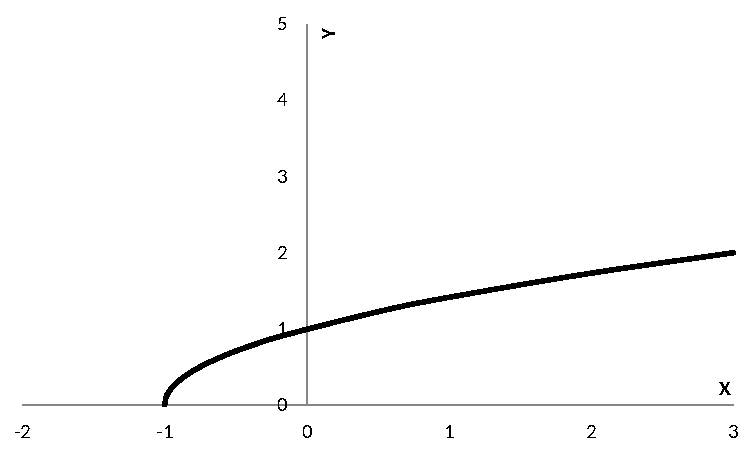
\includegraphics[width=3.49in,height=2.46in]{capitulos/outras_funcoes/media/image8.pdf}
	\end{Center}
\end{figure}

~~

Pode-se observar que: 

\begin{enumerate}
	\item será possível calcular os valores de \textit{y}~, apenas para  \textit{x+1 $ \geq $  0},~ ou \textit{x $ \geq $  -1}. Portanto: \textit{Df(x)=$ \{ $  x $ \in \mathbb{R} $  \textbf{ }/ x $ \geq $  -1$ \} $ .}

	\item  não existirá \textit{y < 0} pois todas as raízes quadradas serão nulas ou positivas. Portanto: \textit{I\textsubscript{m}f(x)=$ \{ $ y $ \in \mathbb{R} $   / y $ \geq $  0$ \} $  }\qedsymbol{} 
\end{enumerate}
\end{texemplo}

\begin{texemplo}
	
Faça o gráfico, determine o domínio e a imagem da função

\quad \quad   \( f \left( x \right) = \left( x-1 \right) ^{1,86} \) .

\textbf{Solução:} É um caso semelhante ao Ex. 2.5 porém com uma subtração. O efeito no gráfico é um deslocamento de uma unidade, neste caso para a direita, do gráfico da função  \( f \left( x \right) = \left( x \right) ^{1,86} \) .

\begin{figure}[H]
	\begin{Center}
		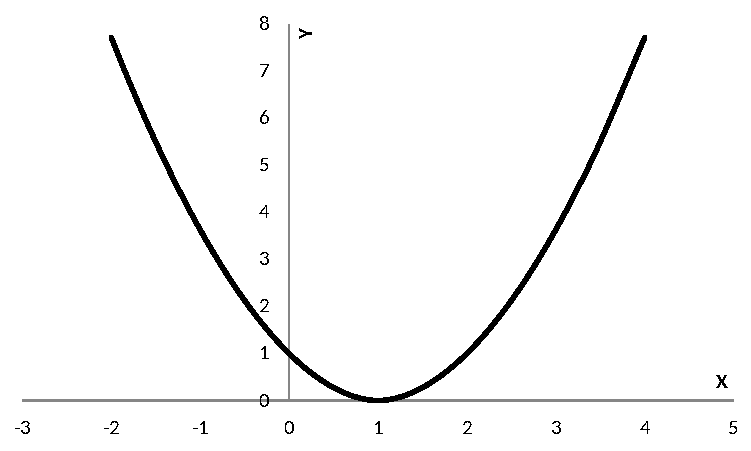
\includegraphics[width=3.57in,height=2.1in]{capitulos/outras_funcoes/media/image9.pdf}
	\end{Center}
\end{figure}

~~

Temos a opção de escrever \textit{f(x)} com expoente fracionário  \( f \left( x \right) =\sqrt[100]{ \left( x-1 \right) ^{186}} \) . Podemos observar que: 

\begin{enumerate}
	\item será possível calcular os valores de \textit{y} para qualquer  \textit{x } real, pois o expoente da base do radicando é um número par. Portanto: \textit{Df(x)=$ \{ $  x $ \in \mathbb{R} $  \textbf{ }$ \} $ .}

	\item não existirá \textit{y < 0} pois todas as raízes serão nulas ou positivas, já que o índice é par. Portanto: \textit{I\textsubscript{m}f(x)=$ \{ $ y $ \in \mathbb{R} $   / y $ \geq $  0$ \} $  }\qedsymbol{} 
\end{enumerate}
\end{texemplo}

\begin{exercicios}
	\exitem{}  Escreva as funções potência na forma de expoente fracionário e como raízes:
	\begin{multicols}{3}

		a) \textit{y = x\textsuperscript{0,2\quad }}
		
		b) \textit{y = x\textsuperscript{1,5}}\textsuperscript{}

		c) \textit{y = x\textsuperscript{1,3333... }}
		
		d) \textit{y = x\textsuperscript{0,75\quad }}

		e) \textit{y = x\textsuperscript{0,12121212...}}

		f) \textit{y = x\textsuperscript{2,5}}
	\end{multicols}

	\exitem{} Determine o domínio e a imagem das funções:

\begin{multicols}3
	
	a) \textit{y = x\textsuperscript{4/3}}

	b) \textit{y = x\textsuperscript{5,5}}
	
	c) \textit{y =(x+2)\textsuperscript{1,3333...}}

	d) \textit{y = (x-3)\textsuperscript{1,25\quad }}
	
	e) \textit{y = (2x-3)\textsuperscript{3/4}}

	f) \textit{y = (x+4)\textsuperscript{2,25}}
\end{multicols}

	\exitem{} Faça manualmente o gráfico das funções do Ex. 2 .

	\exitem{} Faça o gráfico das funções do Ex. 2, usando uma planilha eletrônica.

	\exitem{} Determine os intervalos em que as funções são crescentes ou decrescentes:

	\begin{multicols}{2}
	
	a) \textit{y = x\textsuperscript{3/5\quad }}

	b) \textit{y =(x+2)\textsuperscript{0,5~ }}

	c) \textit{y = (2x+3)\textsuperscript{3/4}}
	
	\end{multicols}
	
	\exitem{} Considere que a função  \( f \left( x \right) =Ax^{m} \) passa pelos pontos \textit{P\textsubscript{1}=(1,1)} e \textit{P\textsubscript{2}=(3,2)} . Substitua as coordenadas dos pontos dados na função e determine os valores de \textit{A} e \textit{m}. 

\end{exercicios}
\section{Funções Racionais}
 
\begin{caixa}
	\begin{tdefinicao}
		Sejam \textit{p(x)} e \textit{q(x)} funções reais. A função é chamada racional se na sua forma irredutível, apresenta a variável no denominador. 
		\( f \left( x \right) =\frac{p \left( x \right) }{q \left( x \right) } \), sendo \(  q \left( x \right)  \neq 0. \) \quad \quad \quad \quad \quad (3.1)
	\end{tdefinicao}
\end{caixa}
\begin{texemplo}

Faça o gráfico, determine o domínio e a imagem da função  \( f \left( x \right) =\frac{1}{x} \).

\textbf{Solução}: A função dada é uma função racional (\textit{p(x)=1} e \textit{q(x)=x}), pois apresenta a variável no denominador. Atribuindo valores para \textit{x,} obtemos os valores de \textit{f(x)} com o uso de uma calculadora. Observemos que \textit{x $ \neq $  0}, pois 1/0 é uma impossibilidade.

\begin{figure}[H]
	\begin{Center}
		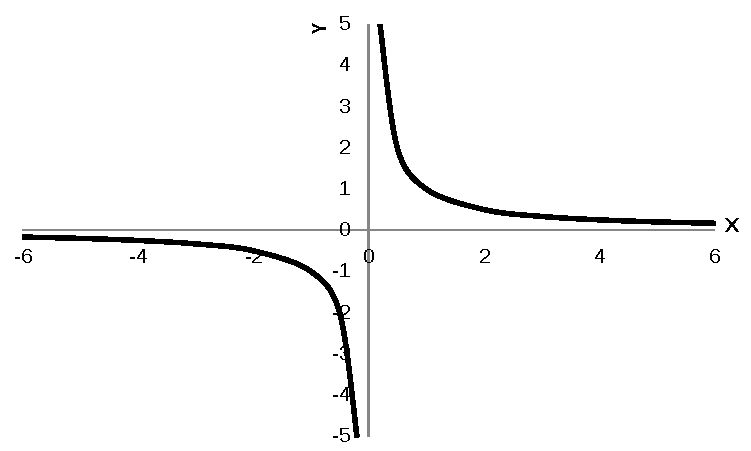
\includegraphics[width=3.14in,height=2.14in]{capitulos/outras_funcoes/media/image10.pdf}
	\end{Center}
\end{figure}

~~

\begin{enumerate}[label=(\roman*)]
	\item Como o denominador não pode ser nulo, \textit{f(0)} não existe. Para qualquer outro valor de \textit{x} a função existe, pois é \textit{1/x}, para \textit{x $ \in \mathbb{R} $  } / \textit{x $ \neq $  0}, é um número real. Portanto,  

\quad \quad \quad \textit{Df(x)=$ \{ $  x $ \in \mathbb{R} $  \textbf{ }/ x $ \neq $  0\textbf{ }$ \} $ .}

	\item Para que \textit{y} seja nulo, o numerador precisaria ser nulo e o denominador não nulo. Portanto, \textit{I\textsubscript{m}f(x)=$ \{ $ y $ \in \mathbb{R} $   / y $ \neq $  0$ \} $  }\qedsymbol{} 
\end{enumerate}

\end{texemplo}
\subsection{Assíntotas horizontais e verticais}

Na função do \textbf{Exemplo 3.1}:

\begin{enumerate}[label=(\roman*)]
	\item Se aumentamos o valor de \textit{x} infinitamente, os valores de \textit{y} tendem a \textit{0}, com valores positivos. Observe que por mais que \textit{x} cresça, a função nunca será zero. (Veja as tabelas)

	\item Se diminuirmos o valor de \textit{x} infinitamente, os valores de \textit{y} tendem a \textit{0}, com valores negativos. Observe que por mais que \textit{x} decresça, a função nunca será zero. (Veja as tabelas)
\end{enumerate}

\begin{multicols}{3}

\begin{table}[H]
 	\centering
\begin{tabular}{p{0.47in}p{0.49in}}
\hline
%row no:1
\multicolumn{1}{|p{0.47in}}{X} & 
\multicolumn{1}{|p{0.49in}|}{Y} \\
\hhline{--}
%row no:2
\multicolumn{1}{|p{0.47in}}{1} & 
\multicolumn{1}{|p{0.49in}|}{1} \\
\hhline{--}
%row no:3
\multicolumn{1}{|p{0.47in}}{10} & 
\multicolumn{1}{|p{0.49in}|}{0,1} \\
\hhline{--}
%row no:4
\multicolumn{1}{|p{0.47in}}{100} & 
\multicolumn{1}{|p{0.49in}|}{0,01} \\
\hhline{--}
%row no:5
\multicolumn{1}{|p{0.47in}}{1000} & 
\multicolumn{1}{|p{0.49in}|}{0,001} \\
\hhline{--}
%row no:6
\multicolumn{1}{|p{0.47in}}{10000} & 
\multicolumn{1}{|p{0.49in}|}{0,0001} \\
\hhline{--}

\end{tabular}
\end{table}

\begin{table}[H]
 			\centering
\begin{tabular}{p{0.47in}p{0.49in}}
\hline
%row no:1
\multicolumn{1}{|p{0.47in}}{X} & 
\multicolumn{1}{|p{0.49in}|}{Y} \\
\hhline{--}
%row no:2
\multicolumn{1}{|p{0.47in}}{-1} & 
\multicolumn{1}{|p{0.49in}|}{-1} \\
\hhline{--}
%row no:3
\multicolumn{1}{|p{0.47in}}{-10} & 
\multicolumn{1}{|p{0.49in}|}{-0,1} \\
\hhline{--}
%row no:4
\multicolumn{1}{|p{0.47in}}{-100} & 
\multicolumn{1}{|p{0.49in}|}{-0,01} \\
\hhline{--}
%row no:5
\multicolumn{1}{|p{0.47in}}{-1000} & 
\multicolumn{1}{|p{0.49in}|}{-0,001} \\
\hhline{--}
%row no:6
\multicolumn{1}{|p{0.47in}}{-10000} & 
\multicolumn{1}{|p{0.49in}|}{-0,0001} \\
\hhline{--}

\end{tabular}
 \end{table}

\end{multicols}

Nesse caso, a reta horizontal \textit{y = 0} é chamada de \textbf{\textit{assíntota horizontal}}.

Ainda na função do \textbf{Exemplo 3.1}:

\begin{enumerate}[label=(\roman*)]
	\item Se atribuirmos valores a \textit{x} cada vez mais próximos a zero, pela direita de zero, observaremos que \textit{y }tende a infinito positivo. (Veja as tabelas)

	\item Se atribuirmos valores a \textit{x} cada vez mais próximos a zero, pela esquerda de zero, observaremos que \textit{y }tende a infinito negativo. (Veja as tabelas)
\end{enumerate}

\begin{table}[H]
 	\centering
\begin{tabular}{p{0.47in}p{0.49in}}
\hline
%row no:1
\multicolumn{1}{|p{0.47in}}{X} & 
\multicolumn{1}{|p{0.49in}|}{Y} \\
\hhline{--}
%row no:2
\multicolumn{1}{|p{0.47in}}{0,9} & 
\multicolumn{1}{|p{0.49in}|}{1,11...} \\
\hhline{--}
%row no:3
\multicolumn{1}{|p{0.47in}}{0,5} & 
\multicolumn{1}{|p{0.49in}|}{2} \\
\hhline{--}
%row no:4
\multicolumn{1}{|p{0.47in}}{0,1} & 
\multicolumn{1}{|p{0.49in}|}{10} \\
\hhline{--}
%row no:5
\multicolumn{1}{|p{0.47in}}{0,01} & 
\multicolumn{1}{|p{0.49in}|}{100} \\
\hhline{--}
%row no:6
\multicolumn{1}{|p{0.47in}}{0,001} & 
\multicolumn{1}{|p{0.49in}|}{1000} \\
\hhline{--}
%row no:7
\multicolumn{1}{|p{0.47in}}{ X} & 
\multicolumn{1}{|p{0.49in}|}{Y} \\
\hhline{--}
%row no:8
\multicolumn{1}{|p{0.47in}}{-0,9} & 
\multicolumn{1}{|p{0.49in}|}{-1,11...} \\
\hhline{--}
%row no:9
\multicolumn{1}{|p{0.47in}}{-0,5} & 
\multicolumn{1}{|p{0.49in}|}{-2} \\
\hhline{--}
%row no:10
\multicolumn{1}{|p{0.47in}}{-0,1} & 
\multicolumn{1}{|p{0.49in}|}{-10} \\
\hhline{--}
%row no:11
\multicolumn{1}{|p{0.47in}}{-0,01} & 
\multicolumn{1}{|p{0.49in}|}{-100} \\
\hhline{--}
%row no:12
\multicolumn{1}{|p{0.47in}}{-0,001} & 
\multicolumn{1}{|p{0.49in}|}{-1000} \\
\hhline{--}

\end{tabular}
\end{table}

Nesse caso, a reta vertical \textit{x = 0} é chamada de \textbf{\textit{assíntota vertical}}.

\begin{texemplo}
Faça o gráfico, determine o domínio e a imagem da função  \( f \left( x \right) =\frac{1}{x-1} \) .

\textbf{Solução}: A função dada é semelhante ao Exemplo 3.1, porém com uma subtração no denominador. Como o denominador não pode ser nulo, a função não existirá para \textit{x = 1}, com o gráfico ficando deslocado de uma unidade para a direita, em relação aquele exemplo.

\begin{figure}[H]
	\begin{Center}
		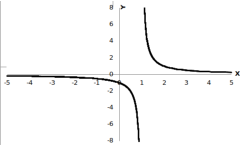
\includegraphics[width=3.6in,height=2.33in]{capitulos/outras_funcoes/media/image11.pdf}
	\end{Center}
\end{figure}

~~

\quad Examinando o gráfico é fácil concluir que : 

\textit{Df(x)=$ \{ $  x $ \in \mathbb{R} $  \textbf{ }/ x $ \neq $  1\textbf{ }$ \} $ ~ } \quad e~~~  \textit{I\textsubscript{m}f(x)=$ \{ $ y $ \in \mathbb{R}$   / y $ \neq $  0$ \} $  }. 

A assíntota horizontal é \textit{y = 0} e a vertical é \textit{x = 1}~~ \qedsymbol{} 
\end{texemplo}

\begin{texemplo}
Faça o gráfico, determine o domínio e a imagem da função  \( f \left( x \right) =\frac{2}{x^{2}-1} \) .

\textbf{Solução}: Como o denominador não pode ser nulo, a função não será definida para \textit{x = +1 }e\textit{ -1}.  A função não interceptará as retas verticais \textit{x = +1 }e\textit{ x=-1. }Fazendo \textit{x = 0}, temos \textit{f(0) = -2}. Com auxílio de uma calculadora podemos investigar mais pontos nos três intervalos:~ \textit{x < -1};~~ \textit{-1 < x < +1}~~~e  \textit{x > 1}, obtendo o gráfico mostrado na figura abaixo. 

\begin{figure}[H]
	\begin{Center}
		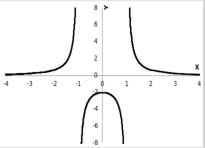
\includegraphics[width=3.55in,height=2.55in]{capitulos/outras_funcoes/media/image12.pdf}
	\end{Center}
\end{figure}

~~

\quad Examinando o gráfico é fácil concluir que: 

\quad \textit{Df(x)=$ \{ $  x $ \in \mathbb{R} $  \textbf{ }/ x $ \neq $  -1} ~e  \textit{x $ \neq $  +1\textbf{ }$ \} $ ~ } e~~~  \textit{I\textsubscript{m}f(x)=$ \{ $ y $ \in \mathbb{R} $   / y $ \leq $  -2 }ou\textit{ y > 0$ \} $ }. Observemos que não existe imagem em~ \textit{-2 < y $ \leq $  0}~ .

\quad As assíntotas verticais serão \textit{x = -1}~ e~ \textit{x = +1}~~~e a horizontal  \textit{y = 0} \textit{ }\qedsymbol{} 
\end{texemplo}

\begin{texemplo}
Faça o gráfico, determine o domínio e a imagem da função  \( f \left( x \right) =\frac{x+1}{x-1} \) .

\textbf{Solução}: Como o denominador não pode ser nulo, a função não será definida para \textit{x=+1}. A função não interceptará a reta vertical \textit{x = +1 }(\textit{assíntota vertical})\textit{. }A função interceptará Y em \textit{y=-1}, pois \textit{f(0) = -1}. Com auxílio de uma calculadora, podemos investigar mais pontos, especificamente quando \textit{x} aumenta infinitamente. Observe que neste caso, y tende a 1, com valores maiores do que 1. Se \textit{x} diminui (tende a menos infinito), observamos que \textit{y} tende a \textit{1}, com valores menores que \textit{1}. Desses dados, podemos concluir que \textit{y = 1} é uma \textit{assíntota horizontal}. Levando estas informações para o plano cartesiano, obtemos o gráfico apresentado pela figura abaixo.

\begin{figure}[H]
	\begin{Center}
		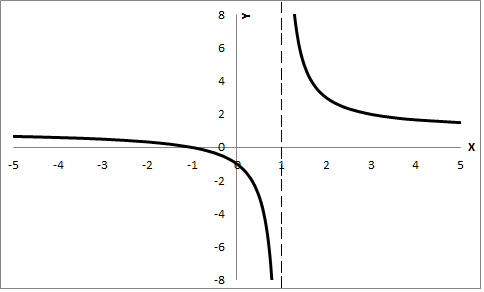
\includegraphics[width=3.86in,height=2.74in]{capitulos/outras_funcoes/media/image13.png}
	\end{Center}
\end{figure}

~~

\quad Examinando o gráfico é fácil concluir que: 

\quad \textit{Df(x)=$ \{ $  x $ \in \mathbb{R} $  \textbf{ }/ x $ \neq $  1} \textit{$ \} $ ~ } e~~~~ \textit{I\textsubscript{m}f(x)=$ \{ $ y $ \in \mathbb{R} $   / y $ \neq $  1$ \} $ }. 

\quad A assíntota vertical será~~ \textit{x = +1}~~~e a horizontal  \textit{y = 1} \textit{  }\qedsymbol{} 
\end{texemplo}

\begin{texemplo}	
Faça o gráfico, determine o domínio e a imagem da função  \( f \left( x \right) =\frac{x^{2}-9}{x-3} \) .

\begin{justify}
\textbf{Solução}: Podemos fatorar o numerador da função e cancelar o fator \textit{(x-3)}, obtendo outra função que chamaremos de \textit{g(x)}.
\end{justify}

\begin{justify}
\quad \quad  \( f \left( x \right) =\frac{ \left( x-3 \right)  \cdot  \left( x+3 \right) }{x-3} \) ~~~~~~~ e~~~  \( g \left( x \right) =x+3 \) 
\end{justify}

\begin{justify}
Observemos que \textit{f(x)} e \textit{g(x)} são perfeitamente iguais para qualquer valor de \textit{x}, exceto para \textit{x = 3}. Teste essa afirmação para diferentes valores de \textit{x}, tais como, \textit{0, 1, -1, -3} e outros. Para~ \textit{x = 3}~~ temos \textit{f((3) = 0/0} que é uma \textbf{indeterminação }(não existe um número \textit{n} tal que \textit{n = 0/0}) e \textit{g(3) = 6}. Portanto, \textit{f((3)~$ \neq $   g(3).}
\end{justify}

\begin{figure}[H]
	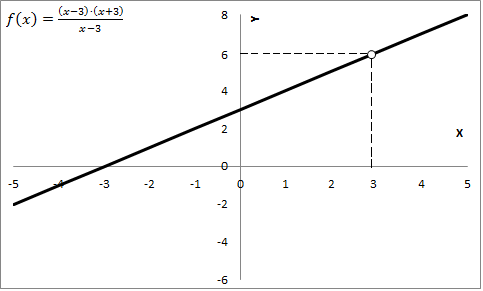
\includegraphics[width=0.45\textwidth]{capitulos/outras_funcoes/media/image14.png} 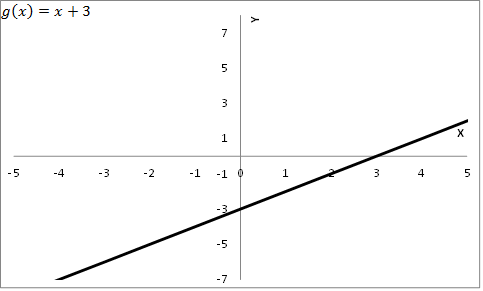
\includegraphics[width=0.45\textwidth]{capitulos/outras_funcoes/media/image15.png}
\end{figure}

\begin{justify}
Analisando os gráficos podemos afirmar que:
\end{justify}

\begin{justify}
\quad  \textit{Df(x)=$ \{ $ x $ \in \mathbb{R} $  \textbf{ }/  x $ \neq $  3$ \} $ }~~~e~  \textit{I\textsubscript{m}f(x)=$ \{ $ y $ \in \mathbb{R} $   / y $ \neq $   6$ \} $ }.
\end{justify}

\begin{justify}
\textit{\quad Dg(x)=$ \{ $ x $ \in \mathbb{R} $  $ \} $ }~~~e~  \textit{I\textsubscript{m}g(x)=$ \{ $ y $ \in \mathbb{R} $  $ \} $ }.
\end{justify}

\quad Assim, as funções \textit{f(x)} e \textit{g(x)} são muito semelhantes mas não são idênticas. Diferem apenas em um ponto:~ \textit{(3,6)}~ \qedsymbol{} 

\end{texemplo}
\newpage
\begin{exercicios}
	\exitem{} Faça o gráfico manualmente, determine o domínio e a imagem das funções:~ 

\begin{multicols}{3}

	a) \( f \left( x \right) =-\frac{3}{x} \)

	b) \( g \left( x \right) =\frac{1}{x-2} \)

	c)  \( h \left( x \right) =\frac{x+1}{x} \)

	d)  \( H \left( x \right) =\frac{x-1}{x+1} \)

	e)  \( F \left( x \right) =\frac{2}{x^{2}-1} \) 

	f)  \( M \left( x \right) =\frac{2}{x^{2}+2x+1} \) 
\end{multicols}

	\exitem{} Faça os gráficos das funções do Ex.1 utilizando uma planilha eletrônica (ou outro programa computacional) 

	\exitem{} Verifique se as funções racionais podem ser reduzidas a funções mais simples. Faça o gráfico e discuta sobre o domínio e a imagem de ambas.

\begin{multicols}{3}
	a) \( f \left( x \right) =\frac{x^{2}-1}{x-1} \)

	b) \( g \left( x \right) =\frac{x^{2}-4x+4}{x-2} \)
	
	c)  \( R \left( x \right) =\frac{x-1}{x^{2}-x} \)

	d)  \( H \left( x \right) =\frac{x^{2}+2x}{x} \)
	
	e) \( q \left( x \right) =\frac{-x^{2}-x}{x^{2}-1} \)

	f)  \( P \left( x \right) =\frac{x^{2}+4x+3}{x+3} \)
\end{multicols}

	\exitem{} Determine as assíntotas horizontais e verticais das funções, se existirem:
\begin{multicols}{3}
a)  \( f \left( x \right) =\frac{5}{-x+1} \)

b)  \( h \left( x \right) =\frac{x-1}{2x} \)

c)  \( g \left( x \right) =\frac{1-x}{x-2} \) 
\end{multicols}
	\exitem{} Faça os gráficos das funções do Ex.4 utilizando uma planilha eletrônica (ou outro programa computacional) e determine o domínio e a imagem.

\end{exercicios}

\section{Funções polinomiais com grau maior do que dois}
\begin{caixa}
\begin{tdefinicao}

As funções polinomiais têm a forma de polinômios de uma incógnita:

 \( f \left( x \right) =a_{0}+a_{1}x+a_{2}x^{2}+a_{3}x^{3}+a_{4}x^{4}+ \ldots +a_{n}x^{n} \) \begin{flushright}(4.1)\end{flushright}

sendo \textit{a\textsubscript{i}} $ \in \mathbb{R} $ e \textit{n = 1,2,3,4, ...}
\end{tdefinicao}
\end{caixa}
O grau de uma função polinomial é o grau do maior expoente da variável. Assim,

 \( f \left( x \right) =5-2x \) é uma função de 1º grau

 \( g \left( x \right) = 1-5x+2x^{2} \) é uma função do 2º grau

 \( h \left( x \right) = -4+x+2x^{2}+x^{3}+x^{4} \) é uma função do 4º grau e assim por diante.

\begin{justify}
\quad As funções polinomiais são contínuas e existem para qualquer número real, pois as operações envolvidas (adição e multiplicação) com as variáveis não apresentam exceções, como as funções racionais (o denominador deve ser positivo) e as potências (se o índice é par, o radicando deve ser positivo). Assim, o domínio será \textit{Df(x)=$ \{ $ x $ \in \mathbb{R} $  \textbf{ }$ \} $ }. 
\end{justify}

\begin{justify}
\quad A imagem das funções polinomiais depende da existência de pontos de máximo ou mínimo, que serão estudados em Cálculo. Neste estágio podemos determinar apenas casos específicos.
\end{justify}

\begin{texemplo}
	
Faça o gráfico, determine o domínio e a imagem da função  \( f \left( x \right) =x^{3} \) .

\begin{justify}
\textbf{Solução}: Podemos construir o gráfico obtendo pontos da função aleatoriamente. Porém, observando a expressão da função, vemos que: 
\end{justify}

\begin{enumerate}[label=(\roman*)]
    \item Quanto maior o valor de \textit{x}, maior será o de \textit{f(x) }.

	\item Se \textit{x} é negativo,~ \textit{f(x) }também será.
\end{enumerate}
\begin{figure}[H]
	\begin{Center}
		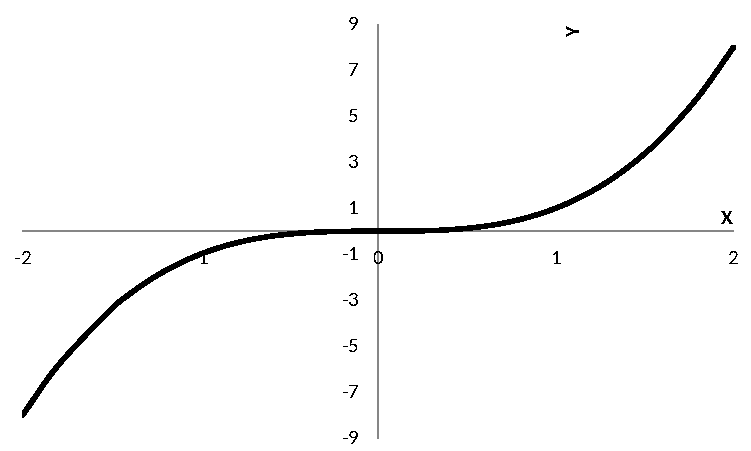
\includegraphics[width=3.46in,height=2.22in]{capitulos/outras_funcoes/media/image16.pdf}
	\end{Center}
\end{figure}

~~

\begin{justify}
O domínio será \textit{Df(x)=$ \{ $ x $ \in \mathbb{R} $  \textbf{ }$ \} $ } e a imagem  \textit{I\textsubscript{m}f(x)=$ \{ $ y $ \in \mathbb{R} $ \textbf{ }$ \} $ } \qedsymbol{}
\end{justify}
\end{texemplo}

\begin{texemplo}
Faça o gráfico, determine o domínio e a imagem da função $$ f ( x ) =x^{3}+1 $$

\begin{justify}
\textbf{Solução}: A expressão desta função é a mesma do exemplo anterior, acrescida de 1.
\quad Portanto, basta acrescentar \textit{1} a cada \textit{y}. (ou levantar a função  \( f \left( x \right) =x^{3} \) em uma unidade)
\end{justify}

\begin{figure}[H]
	\begin{Center}
		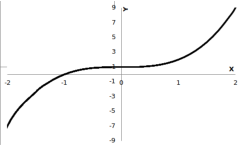
\includegraphics[width=3.62in,height=2.27in]{capitulos/outras_funcoes/media/image17.pdf}
	\end{Center}
\end{figure}

~~

\begin{justify}
O domínio será \textit{Df(x)=$ \{ $ x $ \in \mathbb{R} $  \textbf{ }$ \} $ } e a imagem  \textit{I\textsubscript{m}f(x)=$ \{ $ y $ \in \mathbb{R} \} $ } \qedsymbol{}
\end{justify}
\end{texemplo}

\begin{texemplo}
Faça o gráfico, determine o domínio e a imagem da função 

\quad  $$ g \left( x \right) = \left( x+1 \right) ^{3}$$.

\begin{justify}
\textbf{Solução}: Novamente podemos comparar as expressões das funções desse exemplo com o Exemplo 4.1. Observemos que a base da potência é a diferença. Ou seja, a função \textit{g(x)} é a \textit{f(x)} deslocada uma unidade para a esquerda,
\end{justify}

\begin{figure}[H]
	\begin{Center}
		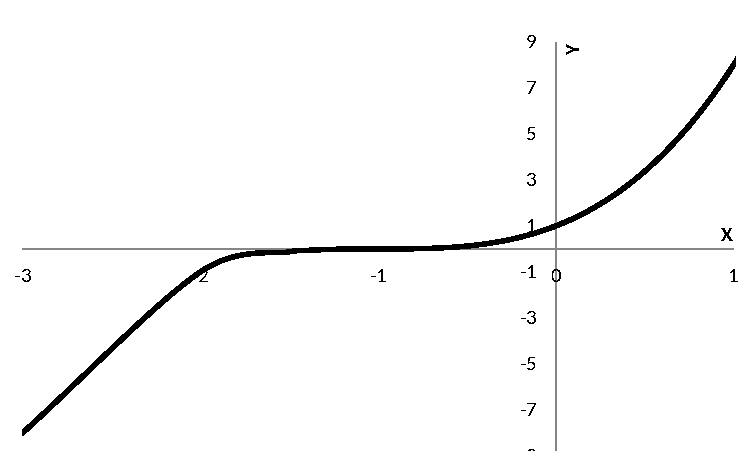
\includegraphics[width=3.65in,height=2.41in]{capitulos/outras_funcoes/media/image18.pdf}
	\end{Center}
\end{figure}

~~

\begin{justify}
O~domínio~será   \textit{Df(x)=$ \{ $ x $ \in \mathbb{R} $  \textbf{ }$ \} $ }~~~e a imagem  \textit{I\textsubscript{m}f(x)=$ \{ $ y $ \in \mathbb{R} $  $ \} $ }~ \qedsymbol{}
\end{justify}
\end{texemplo}

\begin{texemplo}
Faça o gráfico, determine o domínio e a imagem da função 

\quad  $ f \left( x \right) =x^{4}$.

\begin{justify}
\textbf{Solução}: Podemos construir o gráfico obtendo pontos da função aleatoriamente. Porém, observando a expressão da função, vemos que: 
\end{justify}

\begin{enumerate}[label=(\roman*)]
	\item Quanto maior o valor de \textit{x}, maior será o de \textit{f(x) }. 

	\item A função é simétrica em relação ao eixo Y, pois \textit{f(x) = f(-x).} 

	\item  Não existe~ \textit{f(x) < 0 }, pois o expoente de \textit{x} é par.
\end{enumerate}

\begin{figure}[H]
	\begin{Center}
		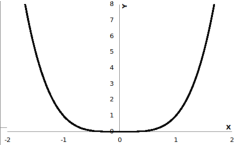
\includegraphics[width=3.54in,height=2.34in]{capitulos/outras_funcoes/media/image19.pdf}
	\end{Center}
\end{figure}

~~

O domínio será \textit{Df(x)=$ \{ $ x $ \in \mathbb{R} $  \textbf{ }$ \} $ } e a imagem \textit{I\textsubscript{m}f(x)=$ \{ $ y $ \in \mathbb{R} $  \textbf{ }/ y > 0$ \} $ } \qedsymbol{}

\end{texemplo}

\begin{texemplo}

Faça o gráfico, determine o domínio e a imagem da função 

\quad  \( f \left( x \right) =x^{4}+3x^{2} \) .

\begin{justify}
\textbf{Solução}: Observando a expressão da função, vemos que colocando \textit{x\textsuperscript{3}} em evidência obtemos  \( f \left( x \right) =x^{3} \left( x+3 \right)  \) . Fazendo \textit{f(x) = 0}, temos: 
\end{justify}

\begin{justify}
\quad  \( 0=x^{2} \left( x^{2}+3 \right)  \) .  
\end{justify}

O lado direito desta expressão só será nulo para \textit{x = 0}. Portanto, \textit{f(x)} intercepta \textit{X} em~ \textit{(0,0)}. 

Outros pontos podem ser obtidos atribuindo valores a \textit{x} e calculando os respectivos valores de \textit{f(x)} .

\begin{figure}[H]
	\begin{Center}
		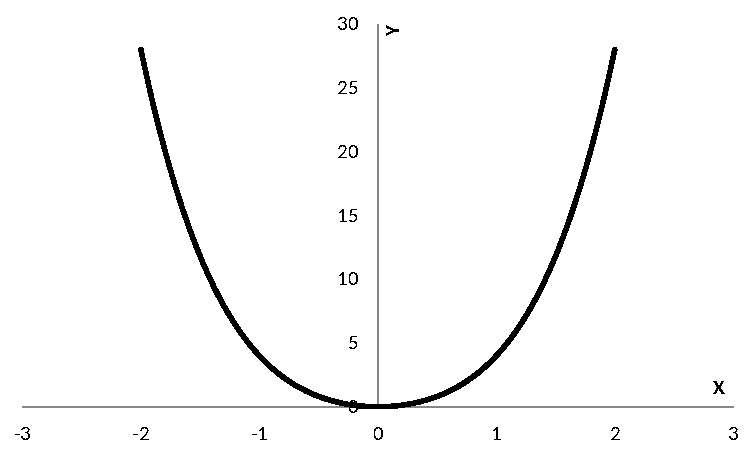
\includegraphics[width=3.61in,height=2.35in]{capitulos/outras_funcoes/media/image20.pdf}
	\end{Center}
\end{figure}

~~

O~domínio~será   \textit{Df(x)=$ \{ $ x $ \in \mathbb{R} $  \textbf{ }$ \} $ }~~~e a imagem  \textit{I\textsubscript{m}f(x)=$ \{ $ y $ \in \mathbb{R} $  \textbf{ }/ y > 0$ \} $ }~ \qedsymbol{}
\end{texemplo}

\begin{texemplo}
Faça o gráfico, determine o domínio e a imagem da função 

\quad  \( f \left( x \right) =x^{3}+x^{2}-2x+3 \) usando uma planilha eletrônica.

\textbf{Solução}: 

\begin{figure}[H]
	\begin{Center}
		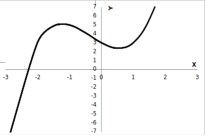
\includegraphics[width=3.57in,height=2.36in]{capitulos/outras_funcoes/media/image21.pdf}
	\end{Center}
\end{figure}

~~

Observando o gráfico, o domínio~será \textit{Df(x)=$ \{ $ x $ \in \mathbb{R} $ \textbf{ }$ \} $ } e a imagem \textit{I\textsubscript{m}f(x)=$ \{ $ y $ \in \mathbb{R} \} $ } \qedsymbol{}

\end{texemplo}

\begin{exercicios}

	\exitem{} Faça o gráfico manualmente das funções:

\begin{multicols}{3}
	a) \( f \left( x \right) =x^{3}+3 \)

	b) \( f \left( x \right) =-x^{3}+3 \)
	
	c)  \( f \left( x \right) =1-2x^{3} \)

	d)  \( f \left( x \right) =x^{3}+3x \)
	
	e)  \( f \left( x \right) =x^{3}+x^{2}-2x \)

	f)  \( g \left( x \right) =x^{4}+3x \) 
\end{multicols}

	\exitem{} Faça o gráfico das funções do Ex.1 usando uma planilha eletrônica e determine o domínio e a imagem.

	\exitem{} Os pontos \textit{P\textsubscript{1}=(0,-1) }e\textit{ P\textsubscript{2}=(2,5)~ }pertencem à função  \( f \left( x \right) =Ax^{3}+B \) \textit{.} Determine os coeficientes \textit{A} e \textit{B} e faça um gráfico da \textit{f(x)}.

	\exitem{} Os pontos \textit{P\textsubscript{1}=(1,-1) }e\textit{ P\textsubscript{2}=(3,-4)~ }pertencem à função  \( g \left( x \right) =Ax^{3}+B \) \textit{.} Determine os coeficientes \textit{A} e \textit{B} e faça um gráfico da \textit{g(x)}.

	\exitem{} Os pontos \textit{P\textsubscript{1}=(0,1),} \textit{P\textsubscript{2}=(1,3) }e\textit{ P\textsubscript{3}=(2,1) }pertencem à função

  \( h \left( x \right) =Ax^{3}+Bx+C \) \textit{.} Determine os coeficientes \textit{A, B} e \textit{C} e faça um gráfico da \textit{h(x)}.

	\exitem{} Os pontos \textit{P\textsubscript{1}=(-1,1),} \textit{P\textsubscript{2}=(0,4) }e\textit{ P\textsubscript{3}=(1,-1) }pertencem à função

  \( q \left( x \right) =Ax^{3}+Bx^{2}+C \) . Determine os coeficientes \textit{A, B} e \textit{C} e faça um gráfico da \textit{q(x)}.

\end{exercicios}

\section{Funções com mais de uma sentença}
\quad Algumas funções podem variar a sentença ao longo do domínio. Vejamos alguns exemplos:

\begin{texemplo}
Faça o gráfico e determine o domínio e a imagem da função

 \[ f \left( x \right) = \left\{ \begin{matrix}
-1, se x<0\\
1 , se x \geq 0.\\
\end{matrix} \right\}
\] 

\textbf{Solução}: A função \textit{f(x)} tem duas sentenças, ambas funções constantes: \textit{f(x)~= - 1  }e\textit{~ f(x)=1. }A primeira vale para \textit{x < 0} e a segunda para \textit{x $ \geq $  0}. Levando estas informações para o gráfico, temos:

\begin{figure}[H]
	\begin{Center}
		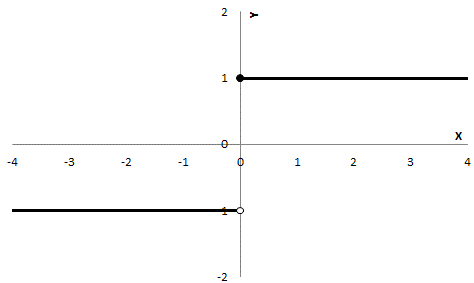
\includegraphics[width=3.66in,height=2.29in]{capitulos/outras_funcoes/media/image22.png}
	\end{Center}
\end{figure}

~~

\quad O domínio e a imagem de \textit{f(x)} são, respectivamente: 

\textit{Df(x)=$ \{ $ x $ \in \mathbb{R} $\textbf{ }$ \} $ } e a imagem  \textit{I\textsubscript{m}f(x)=$ \{ $ y $ \in \mathbb{R} $  }/ \textit{y= -1} e \textit{y=1$ \} $ } \qedsymbol{}
\end{texemplo}

\begin{texemplo}
Em uma cidade, o estacionamento pago depende da hora do dia. Das 8 as 10 h é R$\$$  0,50/h; das 10 as 12 h~ é R$\$$  1,00/h; das 12 as 13 h é grátis; das 13 as 16~h  é R$\$$  1,00/h e das 16 as 118 h é R$\$$  0,50/h. Represente os dados como uma função de \textit{t} (tempo), faça o gráfico e determine o domínio e a imagem.

\textbf{Solução}: Representando estes dados como uma função, temos:

$f \left( t \right) = \left\{ \begin{matrix}
0,50$ se $8 \leq t \leq 10h\\
\begin{matrix}
1,00$ se $10<t \leq 12h\\
\begin{matrix}
0$ se $12<t \leq 13h\\
1,00$ se $13<t \leq 16h\\
\end{matrix}
\\
\end{matrix}
\\
0,50$ se $16<t \leq 18h\\
\end{matrix}\right\}$

\begin{figure}[H]
	\begin{Center}
		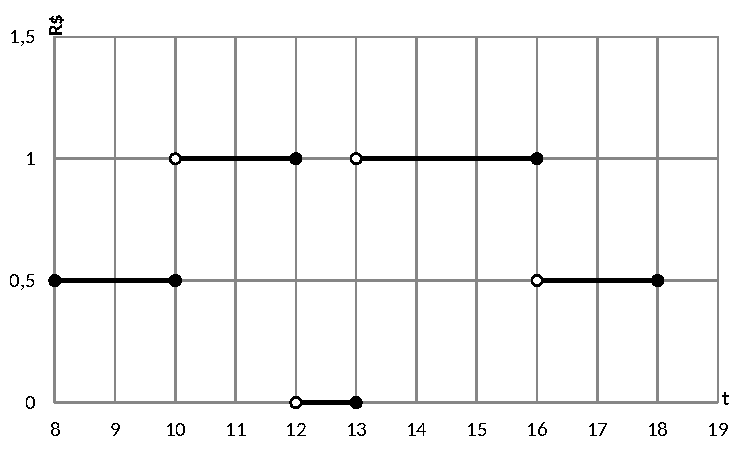
\includegraphics[width=3.91in,height=2.36in]{capitulos/outras_funcoes/media/image23.pdf}
	\end{Center}
\end{figure}

~~

O domínio e a imagem de \textit{f(t)} são, respectivamente: 

\textit{Df(x)=$ \{ $ t $ \in \mathbb{R} $  \textbf{ / 8 < t < 18}$ \} $ }~~~e a imagem  \textit{I\textsubscript{m}f(x)=$ \{ $ y $ \in \mathbb{R} $  }/ \textit{y= 0,5} ; \textit{y=0} e \textit{y=1$ \} $ }~ \qedsymbol{}
\end{texemplo}

\begin{texemplo}
Faça o gráfico e determine o domínio e a imagem da função

 $[ f \left( x \right) = \left\{ \begin{matrix}
-x, $ se $ x<0\\
0 $ se $ x=0\\
\text{x $ se $ x>0}\\
\end{matrix}\right\}
]$ 

\textbf{Solução}: A função \textit{f(x)} tem três sentenças: a reta~ \textit{f(x)~= - x  }para \textit{x < 0}; a função constante\textit{~ f(x)=0~ }para \textit{x = 0}~~e a função identidade  \textit{f(x)~=~ x  }~para  \textit{x > 0}. Levando estas informações para o gráfico, temos:

\begin{figure}[H]
	\begin{Center}
		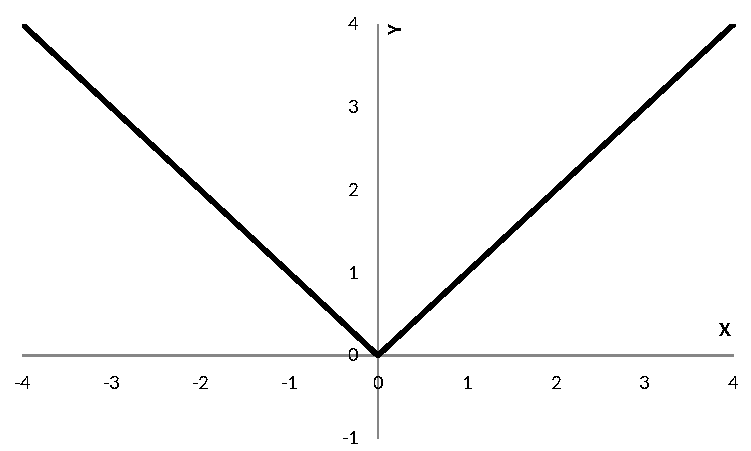
\includegraphics[width=3.54in,height=2.48in]{capitulos/outras_funcoes/media/image24.pdf}
	\end{Center}
\end{figure}

~~

\quad O domínio e a imagem de \textit{f(x)} são, respectivamente: 

\textit{Df(x)=$ \{ $ x $ \in \mathbb{R} $  \textbf{ }$ \} $ }~~~e a imagem  \textit{I\textsubscript{m}f(x)=$ \{ $ y $ \in \mathbb{R} $  } \textit{$ \} $ }~ \qedsymbol{}
\end{texemplo}

\begin{texemplo}
Algumas funções periódicas podem ser escritas especificando suas sentenças para um período que se repete. 

\quad Seja \textit{T} o período: \textit{T = 2}~ \textit{,} da função 

 $[ f \left( x \right) = \left\{ \begin{matrix}
0, $ para $ 0 < x \leq T/2\\
\text{1, $ para $}\frac{T}{2}< x \leq T.\\
\end{matrix}\right\}
]$

\quad Faça o gráfico e determine o domínio e a imagem da função.

\textbf{Solução}: Se o período é \textit{T = 2} , significa que se a função~inicia~em   \textit{x = 0} , se repete de 2 em 2, tanto para a esquerda como para a direita da origem, como mostra o gráfico.

\begin{figure}[H]
	\begin{Center}
		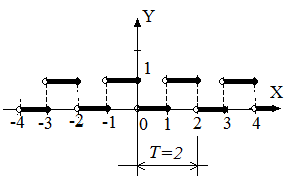
\includegraphics[width=3.15in,height=1.95in]{capitulos/outras_funcoes/media/image25.png}
	\end{Center}
\end{figure}

~~

Esta função é conhecida como \textit{função degrau}. O domínio e a imagem de \textit{f(x)} são, respectivamente: 

\textit{Df(x)=$ \{ $ x $ \in \mathbb{R} $  \textbf{ }$ \} $ }~~~e a imagem  \textit{I\textsubscript{m}f(x)=$ \{ $ y = 0 }e\textit{ y =1$ \} $ } \qedsymbol{}

\end{texemplo}
\begin{exercicios}

	\exitem{} Dada a função  $( f \left( x \right) = \left\{ \begin{matrix}
-2\text{, $ se $ x<0}\\
1 , $ se $ x \geq 0.\\
\end{matrix}\right\}
  )$, determine :

\begin{multicols}{5}
	a) \textit{f(-1})
	
	b) \textit{f(0})
	
	c) \textit{f(-3})
	
	d) \textit{f(1})
	
	e) \textit{f(2})
\end{multicols}

	\exitem{} Faça os gráficos das seguintes funções:

\begin{multicols}{2}
	a) $( f \left( x \right) = \left\{ \begin{matrix}
	-1~ , $ se $ x<0\\
	1 , $ se $ x \geq 0.\\
	\end{matrix}\right\}
  	)$  

	b) $( f \left( x \right) = \left\{ \begin{matrix}
	\text{x~ , $ se $ x<0}\\
	-x , $ se $ x \geq 0.\\
	\end{matrix}\right\}
	)$

	c) $( ~f \left( x \right) = \left\{ \begin{matrix}
	-2~ , $ se $ x \leq 1\\
	\text{3x , $ se $ x>1.}\\
	\end{matrix}\right\}
	)$
	
	d) $( ~~f \left( t \right) = \left\{ \begin{matrix}
	0~, $ se $ t \neq 0\\
	1 , $ se $ t=0.\\
	\end{matrix}\right\}
	)$ 
\end{multicols}

	\exitem{} Faça o gráfico das funções periódicas:

\begin{enumerate}[label=\alph*]
	\item $( f \left( x \right) = \left\{ \begin{matrix}
	-1 , $ se $ 0< x \leq T/2\\
	\text{1~ , $ se $ }\frac{T}{2}< x \leq T.\\
	\end{matrix}\right\}
	)$
	Para\textit{ T = 4}.
	
	\item $( \text{~ f} \left( x \right) = \left\{ \begin{matrix}
	0, $ se $ 0 \leq  x<T/2\\
	\text{1 , $ se $ }\frac{T}{2} \leq  x<T.\\
	\end{matrix}\right\}
	)$
	Para \textit{T = 1}. 
\end{enumerate}

	\exitem{} Faça o gráfico da função "dente de serra", definida por: $( f \left( x \right) = x, $ para $ T = 1 )$ . Determine o domínio e a imagem.

	\exitem{} Faça o gráfico da função~definida por: $( f \left( x \right) =-x+\text{1 ,} $ para $ T=1 )$ . Determine o domínio e a imagem.

	\exitem{} Faça o gráfico da função definida por:

	$( f \left( x \right) = \left\{ \begin{matrix}
	0,~ $ se $ 0<x \leq T/2\\
	x,~~ $ se $  T/2<x \leq T\\
	\end{matrix}\right\}
 	, $ para $ T=2  )$ . Determine o domínio e a imagem.

	\exitem{} A função "modular" é definida por:

	$( f \left( x \right) = \left\{ \begin{matrix}
	x,~ $ se $ x  \geq 0\\
	-x,~~ $ se $  x<0\\
	\end{matrix}\right\}
  	)$.  Determine o domínio e a imagem.

\end{exercicios}
\section{Funções pares e ímpares}
\begin{caixa}
\begin{tdefinicao}

Uma função é \textbf{par} se é simétrica em relação ao eixo Y. 

Ou em linguagem matemática, 

\quad \textit{f(-x) = f(x)~ }, \quad \quad para qualquer \textit{x $ \in $   Df(x)} \qedsymbol{}
\end{tdefinicao}
\end{caixa}

\begin{texemplo}

Verifique se a função \textit{f(x) = x\textsuperscript{2}} -1~~ é par.

\textbf{ Solução}: 

\begin{figure}[H]
	\begin{Center}
		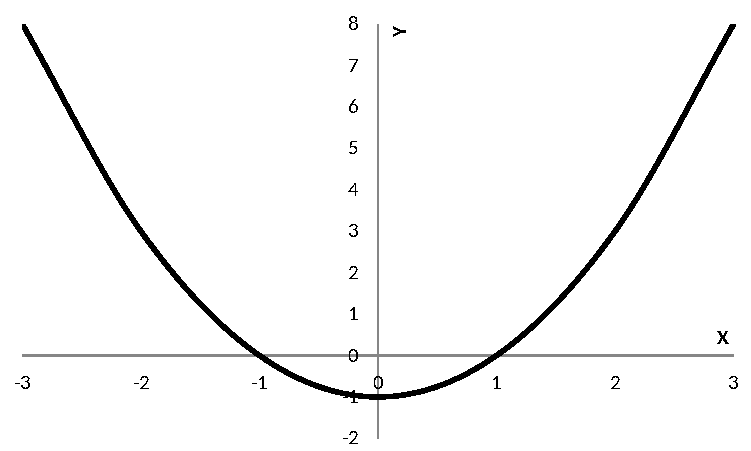
\includegraphics[width=3.53in,height=2.28in]{capitulos/outras_funcoes/media/image26.pdf}
	\end{Center}
\end{figure}

~~

Analisando o gráfico observa-se que~ \textit{f(x)} é uma parábola e que o eixo Y é seu eixo de simetria. Usando a Def. 6.1, observa-se que para qualquer \textit{x $ \in \mathbb{R} $  \textbf{ }}, \textit{f(x) = f(-x).}~ Portanto,~ \textit{f(x)} é uma função par \qedsymbol{}
\end{texemplo}

\begin{caixa}
\begin{tdefinicao}
Uma função é \textbf{ímpar} se é anti-simétrica (simetria com o sinal oposto) em relação ao eixo Y. Ou em linguagem matemática,

	\quad \textit{f(-x) = - f(x)~ }, \quad \quad para qualquer \textit{x $ \in $   Df(x)} \qedsymbol{}
\end{tdefinicao}
\end{caixa}

\begin{texemplo}

Verifique se a função \textit{f(x) = x\textsuperscript{3}} é par ou ímpar.

\textbf{Solução}: 

\begin{figure}[H]
	\begin{Center}
		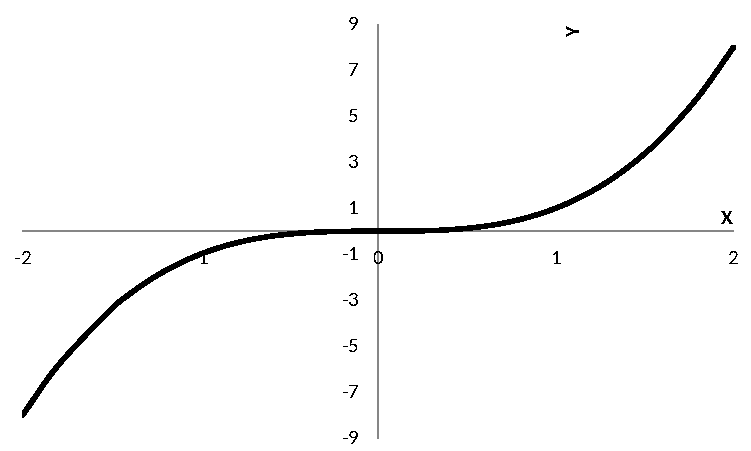
\includegraphics[width=3.65in,height=2.4in]{capitulos/outras_funcoes/media/image27.pdf}
	\end{Center}
\end{figure}

~~

Analisando o gráfico observa-se que~ \textit{f(x)} é antissimétrica em relação ao eixo Y. Usando a Def. 6.1, observa-se que para qualquer \textit{x $ \in \mathbb{R} $ \textbf{ }}, \textit{f(x) = -f(-x).} Portanto, \textit{f(x)} é uma função ímpar \qedsymbol{} 
\end{texemplo}

\begin{exercicios}

	\exitem{} Verifique se as funções são pares e ímpares:

\begin{multicols}{3}
	a) \textit{f(x) =} \textit{-x\textsuperscript{2} + 5}

	b) \textit{f(x) =} \textit{-x\textsuperscript{3}} 
	
	c) \textit{f(x) =} \textit{-x\textsuperscript{4}}

	d) \textit{f(x) =} \textit{x\textsuperscript{5} + 3}
	
	e) \textit{f(x) =} \textit{-5x\textsuperscript{2} +3}

	f) \textit{f(x) =} \textit{3x\textsuperscript{3}}
\end{multicols}

	\exitem{} Verifique se a função abaixo é par ou ímpar:

 	$[ f \left( x \right) = \left\{ \begin{matrix}
	-1~ , $ se $ x<0\\
	0, $ se $ x=0\\
	\text{1 , $ se $ x>0.}\\
	\end{matrix}\right\}
	]$ 

	\exitem{}  Verifique se a função abaixo é par ou ímpar:

	$( f \left( x \right) = \left\{ \begin{matrix}
	x,~ $ se $ x  \geq 0\\
	-x,~~ $ se $  x<0\\
	\end{matrix}\right\}
	)$.

	\exitem{} Crie uma função par, faça o gráfico e determine o domínio e a imagem.

	\exitem{} Crie uma função ímpar, faça o gráfico e determine o domínio e a imagem.

\end{exercicios}
\newpage
\section{Módulo e funções modulares}

\begin{caixa}
\begin{tdefinicao}

O módulo de um número real  \textit{x} é representado por $ \vert $\textit{x}$\vert $  e definido como:

$(  \vert x \vert = \left\{ \begin{matrix}
x, $ se $ x  \geq 0\\
-x, $ se $ x<0\\
\end{matrix}\right\}
  $)\begin{flushright}(7.1)\end{flushright}
\end{tdefinicao}
\end{caixa}

\begin{texemplo}

Determine o módulo de \textit{x = -5}  e \textit{x = 5}.~~ 

\textbf{Solução}: Usando a Def. 7.1, temos:

\quad Para \textit{x = -5}~ , \textit{x < 0}~,~ então  $ \vert $ \textit{x}$ \vert $  \textit{= -(-5) = + 5}.~~~~~ 

\quad Para \textit{x = 5}~ , \textit{x > 0}~,~ então  $ \vert $ \textit{x}$ \vert $  \textit{= +5 }\qedsymbol{}~~~~ 
\end{texemplo}

\begin{texemplo}
	
Determine $ \vert $ \textit{x+3}$ \vert $ .~~ 

\textbf{Solução}: Usando a Def. 7.1, temos:

\quad Se \textit{x+3 $ \geq $  0 , }ou\textit{~x $ \geq $  -3,  }temos\textit{~ }$ \vert $ \textit{x+3}$ \vert $  = \textit{x+3}.

\quad Se \textit{x+3 < 0 , }ou\textit{x < -3,  }temos\textit{}$ \vert $ \textit{x+3}$ \vert $  = -(\textit{x+3) }\qedsymbol{}
\end{texemplo}

\begin{texemplo}
Os módulos podem ser usados para representar intervalos. Quais são os valores de \textit{x} que satisfazem a desigualdade  I =~ $ \vert $ \textit{x}$ \vert $  \textit{< 1}. 

\textbf{Solução}: Usando a Def. 7.1, temos:

\quad Se \textit{x $ \geq $  0 } temos \textit{x < 1}.

\begin{figure}[H]
	\begin{Center}
		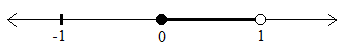
\includegraphics[width=3.6in,height=0.47in]{capitulos/outras_funcoes/media/image28.png}
	\end{Center}
\end{figure}

\quad Se \textit{x< 0 , } temos \textit{-x} < 1 ou \textit{x > -1.}

\begin{figure}[H]
	\begin{Center}
		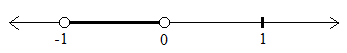
\includegraphics[width=3.61in,height=0.5in]{capitulos/outras_funcoes/media/image29.png}
	\end{Center}
\end{figure}

\quad Unindo os dois intervalos, temos que I =$ \{ $ \textit{ x $ \in \mathbb{R} $  \textbf{ }} / \textit{-1 < x < 1} $ \} $  

\begin{figure}[H]
	\begin{Center}
		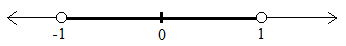
\includegraphics[width=3.6in,height=0.48in]{capitulos/outras_funcoes/media/image30.png}
	\end{Center}
\end{figure}

\qedsymbol{}

\end{texemplo}
\begin{caixa}
\begin{tdefinicao}
Seja \textit{x} uma variável real. Uma função é modular se possui $ \vert $ \textit{ f(x) $ \vert $ } na sua expressão.
\end{tdefinicao}
\end{caixa}

\begin{texemplo}

Faça o gráfico da função modular \textit{f(x) =} $ \vert $ \textit{x}$ \vert $. Determine o domínio e a imagem.  

\textbf{Solução}: Usando a Def. 7.1 temos:

\quad Se \textit{x $ \geq $  0} temos \textit{f(x) = x}.

\quad Se \textit{x< 0 , } temos \textit{f(x) = -x }. Temos duas retas, uma para cada intervalo do domínio.

\begin{figure}[H]
	\begin{Center}
		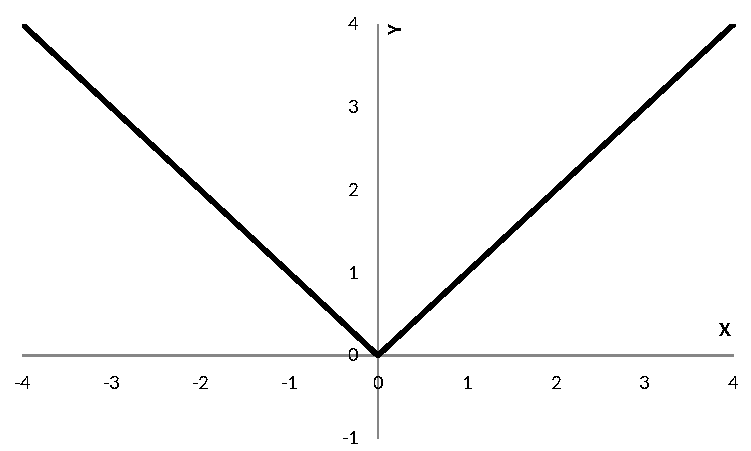
\includegraphics[width=3.64in,height=2.3in]{capitulos/outras_funcoes/media/image24.pdf}
	\end{Center}
\end{figure}

~~

\quad Observando o gráfico, o domínio será   \textit{Df(x)=$ \{ $ x $ \in \mathbb{R} $  \textbf{ }$ \} $ } e a imagem 

\quad  \textit{I\textsubscript{m}f(x)=$ \{ $ y $ \in \mathbb{R} $  }/ \textit{y $ \geq $  0$ \} $ } \qedsymbol{}
\end{texemplo}

\begin{texemplo}

Faça o gráfico da função modular \textit{f(x) =} $ \vert $ \textit{x+1}$ \vert $ . Determine o domínio e a imagem.  

\textbf{Solução}: Usando a Def. 7.1 temos:

\quad Se \textit{x+1 $ \geq $  0} ou \textit{x $ \geq $ -1}temos\textit{f(x) = x+1 }.

\quad Se \textit{x+1 < 0} ou \textit{ x < -1}temos\textit{f(x) = -(x+1)}. Temos duas retas, uma para cada intervalo do domínio.

\begin{figure}[H]
	\begin{Center}
		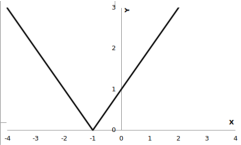
\includegraphics[width=3.65in,height=2.23in]{capitulos/outras_funcoes/media/image31.pdf}
	\end{Center}
\end{figure}

~~

\quad Observando o gráfico, o domínio será   \textit{Df(x)=$ \{ $ x $ \in \mathbb{R} $  \textbf{ }$ \} $ } e a imagem.

\quad \textit{I\textsubscript{m}f(x)=$ \{ $ y $ \in \mathbb{R} $  }/ \textit{y $ \geq $  0$ \} $ } \qedsymbol{}
\end{texemplo}

\begin{texemplo}

Faça o gráfico da função modular \textit{f(x) =} $ \vert $ \textit{x$ \vert $ -1}. Determine o domínio e a imagem.  

\textbf{Solução}: Usando a Def. 7.1 temos:

\quad Se \textit{x $ \geq $  0}temos\textit{~ f(x) = x-1}.

\quad Se \textit{x < 0, }temos\textit{~ f(x) = -x-1}. Temos duas retas, uma para cada intervalo do domínio.

\begin{figure}[H]
	\begin{Center}
		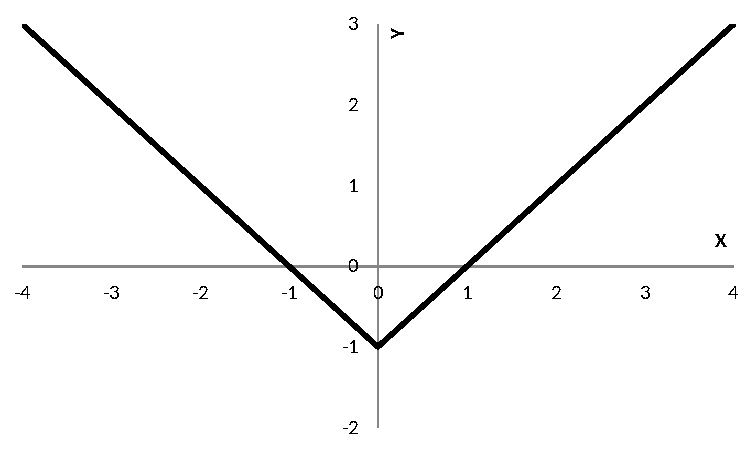
\includegraphics[width=3.55in,height=2.24in]{capitulos/outras_funcoes/media/image32.pdf}
	\end{Center}
\end{figure}

~~

\quad Observando o gráfico, o~domínio~será   \textit{Df(x)=$ \{ $ x $ \in \mathbb{R} $  \textbf{ }$ \} $ } e a imagem

\quad \textit{I\textsubscript{m}f(x)=$ \{ $ y $ \in \mathbb{R} $  }/ \textit{y $ \geq $  -1$ \} $ } \qedsymbol{}
\end{texemplo}

\begin{texemplo}

Faça o gráfico da função modular \textit{f(x) =} $ \vert $ \textit{x\textsuperscript{2}-1$ \vert $ }~. Determine o domínio e a imagem.  

\textbf{Solução}: Usando a Def. 7.1 temos:

\quad Se \textit{x\textsuperscript{2}-1 $ \geq $  0, }

\quad \textit{x\textsuperscript{2}$ \geq $ 1.  }Então, nos intervalos \textit{ x~$ \leq $ -1   }ou~ \textit{~x $ \geq $1} temos \textit{ f(x) =} \textit{x\textsuperscript{2}-1. }

\quad Se \textit{x\textsuperscript{2}-1 < 0}

\quad \textit{x\textsuperscript{2} < 1.  }Então, no intervalo \textit{-1< x < 1}temos\textit{ f(x) =} -\textit{x\textsuperscript{2 } + 1.}

\begin{figure}[H]
	\begin{Center}
		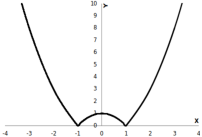
\includegraphics[width=3.55in,height=2.42in]{capitulos/outras_funcoes/media/image33.pdf}
	\end{Center}
\end{figure}

~~

\quad Observando o gráfico, o domínio será   \textit{Df(x)=$ \{ $ x $ \in \mathbb{R} $ \textbf{ }$ \} $ } e a imagem

\quad \textit{I\textsubscript{m}f(x)=$ \{ $ y $ \in \mathbb{R} $  }/ \textit{y $ \geq $  0$ \} $ } \qedsymbol{}
\end{texemplo}

\begin{exercicios}

	\exitem{} Determine os módulos, usando a definição 7.1:

\begin{multicols}{3}
	a) \textit{$ \vert $ -7$ \vert $  = }

	b) \textit{$ \vert $ x+1$ \vert $  = }
	
	c) \textit{$ \vert $ +8$ \vert $  = }
	
	d) \textit{$ \vert $ x-1$ \vert $  = }
	
	e) \textit{$ \vert $ -x+2$ \vert $  = }

	f) \textit{$ \vert $ 5 –x $ \vert $  = }
\end{multicols}

	\exitem{} Determine os intervalos em \textit{x} que satisfazem os módulos:

\begin{multicols}{3}
	a) \textit{$ \vert $ x$ \vert $  > 1}

	b) \textit{$ \vert $ x+1$ \vert $  < 0}
	
	c) \textit{$ \vert $ x$ \vert $  < 1}

	d) \textit{$ \vert $ x-1$ \vert $  < 2} 
	
	e) \textit{$ \vert $ -x+2$ \vert $  < 2}
	
	f) \textit{$ \vert $ 5 –x $ \vert $  < 1}
\end{multicols}

	\exitem{} Desenhe os intervalos do exercício anterior em uma reta real.

	\exitem{} Faça o gráfico das funções e determine o domínio e a imagem.

\begin{multicols}{3}

	a) \textit{F(x)=$ \vert $ -x$ \vert $}

	b) \textit{ f(x)=$ \vert $ 2x-3$ \vert $ }
	
	c) \textit{f(x)=$ \vert $ -2x-3$ \vert $ } 
	
	d) \textit{g(x)=$ \vert $ -x+5$ \vert $}
	
	e) \textit{G(x)=$ \vert $ 1-x$ \vert $ }

	f) \textit{g(t)=$ \vert $  t $ \vert $  +2}

	g) \textit{H(x)=$ \vert $  x\textsuperscript{2 }+4$ \vert $}
	
	h) \textit{F(x)=$ \vert $  -x\textsuperscript{2 }$ \vert $ +5}

	i) \textit{f(t)=$ \vert $  t\textsuperscript{2} +1$ \vert $ -2}
\end{multicols}

	\exitem{} Faça o gráfico em uma planilha eletrônica e determine o domínio e a imagem das funções.

\begin{multicols}{3}

	a) \textit{f(x)=$ \vert $ x\textsuperscript{2 }-x -2$ \vert $}

	b) \textit{g(x)=$ \vert $  x\textsuperscript{2 }-x$ \vert $ +1}
	
	c) \textit{f(x)=$ \vert $ -x\textsuperscript{2 }+4$ \vert $}

	d) \textit{p(t)=$ \vert $ t $ \vert $ + t\textsuperscript{2 }+4}
	
	e) \textit{p(t)=$ \vert $ t $ \vert $ - t\textsuperscript{2 }+2\quad }

	f) \textit{g(x)=$ \vert $  x\textsuperscript{3 }$ \vert $ - x\textsuperscript{2}+1}
\end{multicols}

	\exitem{} Faça o gráfico da função periódica:   \( f \left( x \right) = \vert x \vert   \) , para \textit{T = 1}.

\begin{enumerate}
	\item Considerando que \textit{f(x)} é par.

	\item Considerando que \textit{f(x)} é ímpar.
\end{enumerate}
\end{exercicios}

\newpage
\section{RESPOSTAS DOS EXERCÍCIOS PROPOSTOS}

\begin{respostas}{2}
	\begin{multicols}{2}
	\ansitem{} 
		a) \( x^{1/5};\sqrt[5]{x} \)
	
		b) \( x^{3/2};\sqrt[]{x^{3}} \)  

		c) \( x^{4/3};\sqrt[3]{x^{4}} \)
	
		d) \( x^{3/4};\sqrt[4]{x^{3}} \)

		e) \( x^{4/33};\sqrt[33]{x^{4}} \)
	
		f) \( x^{5/2};\sqrt[]{x^{5}} \) 
	\end{multicols}

	\ansitem{}  a)  \( D= \{ x \in R \} \) \( Im= \{ y \in R/y \geq 0 \}  \) 

	b) \( D= \{ x \in R/x \geq 0 \}  \) \( Im= \{ y \in R/y \geq 0 \} \)

	c) \( D= \{ x \in R \}  \) \( Im= \{ y \in R/y \geq 0 \}  \)

	d) \( D= \{ x \in R/x \geq 3 \}  \) \( Im= \{ y \in R/y \geq 0 \}  \) \( Im= \{ y \in R/y \geq 0 \}  \) 

	e) \( D= \{ x \in R/x \geq 3/2  \}  \) \( Im= \{ y \in R/y \geq 0 \}  \) 

	f)  \( D= \{ x \in R~/x \geq -4 \} \) \( Im= \{ y \in R/y \geq 0 \}  \)
	
\ansitem{} a) \quad

\begin{figure}[H]
	\begin{Center}
		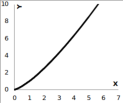
\includegraphics[width=2.57in,height=2.05in]{capitulos/outras_funcoes/media/image34.pdf}
	\end{Center}
\end{figure}

~~

b)\quad 

\begin{figure}[H]
	\begin{Center}
		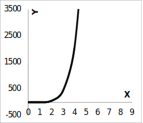
\includegraphics[width=2.47in,height=2.14in]{capitulos/outras_funcoes/media/image35.pdf}
	\end{Center}
\end{figure}

~~

c)\quad 

\begin{figure}[H]
	\begin{Center}
		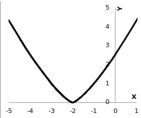
\includegraphics[width=2.46in,height=1.95in]{capitulos/outras_funcoes/media/image36.pdf}
	\end{Center}
\end{figure}

~~

d)

\begin{figure}[H]
	\begin{Center}
		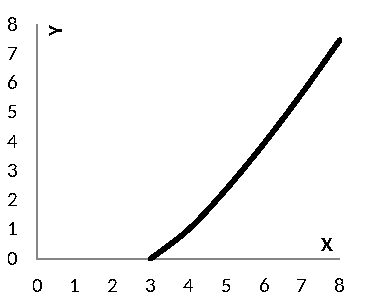
\includegraphics[width=2.46in,height=1.89in]{capitulos/outras_funcoes/media/image37.pdf}
	\end{Center}
\end{figure}

~~

e) \quad 

\begin{figure}[H]
	\begin{Center}
		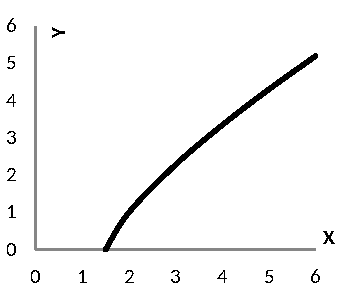
\includegraphics[width=2.46in,height=1.99in]{capitulos/outras_funcoes/media/image38.pdf}
	\end{Center}
\end{figure}

~~

f)

	\begin{figure}[H]
		\begin{Center}
			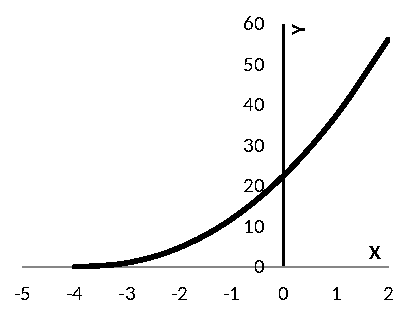
\includegraphics[width=2.42in,height=2.11in]{capitulos/outras_funcoes/media/image39.pdf}
		\end{Center}
	\end{figure}


	\setcounter{enumi}{4}
	\ansitem{} a) \( \text{Crescente para x}  \in R  \)

	b) \( Crescente~para~x>-2 \) \quad 

	c)  \( Crescente~para~x>-1 \) 

	\ansitem{} \( f \left( x \right) =x^{0,6309298} \)  

\end{respostas}

\begin{respostas}{3}

	\ansitem{} a) \( D= \{ x \in R/x \neq 0 \}  \) \\ \( Im= \{ y \in R/y \neq 0 \}  \) 


	\begin{figure}[H]
		\begin{Center}
			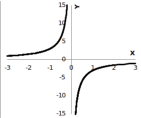
\includegraphics[width=2.66in,height=2.22in]{capitulos/outras_funcoes/media/image40.pdf}
		\end{Center}
	\end{figure}

~~

	b)  \( D= \{ x \in R/x \neq 2 \}  \) \\ \( Im= \{ y \in R/y \neq 0 \}  \) 

	\begin{figure}[H]
		\begin{Center}
			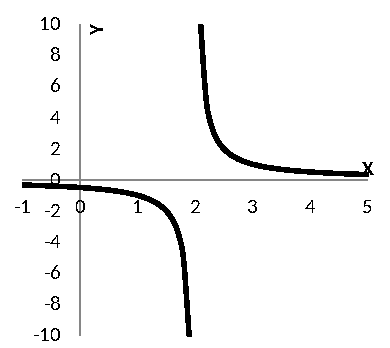
\includegraphics[width=2.66in,height=2.11in]{capitulos/outras_funcoes/media/image41.pdf}
		\end{Center}
	\end{figure}

~~

	c) \( D= \{ x \in R/x \neq 0 \}  \) \\ \( Im= \{ y \in R/y \neq 1 \}  \)

	\begin{figure}[H]
		\begin{Center}
			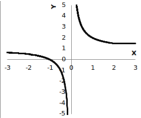
\includegraphics[width=2.65in,height=2.22in]{capitulos/outras_funcoes/media/image42.pdf}
		\end{Center}
	\end{figure}

	d)  \( D= \{ x \in R/x \neq -1 \}\)\\\(Im= \{ y \in R/y \neq 1 \}  \) 

	\begin{figure}[H]
		\begin{Center}
			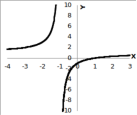
\includegraphics[width=2.6in,height=2.19in]{capitulos/outras_funcoes/media/image43.pdf}
		\end{Center}
	\end{figure}

	e)  \( D= \{ x \in R/x \neq -1 e x \neq 1 \}  \)\\ \( Im= \{ y \in R/y \leq -2 ou y>0 \}  \)

	\begin{figure}[H]
		\begin{Center}
			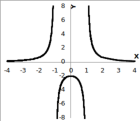
\includegraphics[width=2.66in,height=2.31in]{capitulos/outras_funcoes/media/image44.pdf}
		\end{Center}
	\end{figure}

	f)  \( D= \{ x \in R/x \neq -1 \}  \)\\\( Im= \{ y \in R/y>0 \} \)

	\begin{figure}[H]
		\begin{Center}
			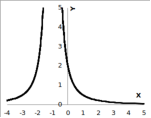
\includegraphics[width=2.92in,height=2.46in]{capitulos/outras_funcoes/media/image45.pdf}
		\end{Center}
	\end{figure}

	\setcounter{enumi}{2}
	\ansitem a) \( f1 \left( x \right) =x+1;  \) \\ \( Df \left( x \right) = \{ x \in R/x \neq 1 \}  \)\\\(Imf \left( x \right) = \{ y \in R/y \neq 2 \} \)

	\begin{figure}[H]
		\begin{Center}
			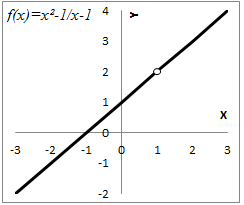
\includegraphics[width=2.62in,height=2.21in]{capitulos/outras_funcoes/media/image46.png}
		\end{Center}
	\end{figure}

	b) \( g \left( x \right) =x-2\) \\ \(D= \{ x \in R \}  \) \\ \( Im= \{ y \in R \}  \)\\ 

	\( g1 \left( x \right) =\frac{x^2-4x+4}{x-2}\)\\\(D= \{ x \in R/x \neq 2 \}  \) \\\( Im= \{ y \in R/y \neq 0 \}\)

	\begin{figure}[H]
		\begin{Center}
			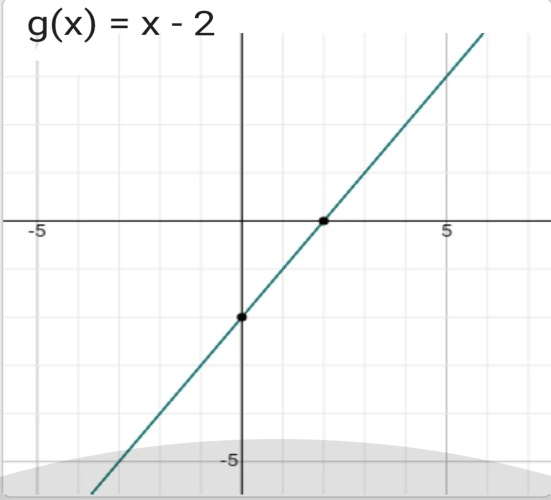
\includegraphics[width=2.5in,height=2.27in]{capitulos/outras_funcoes/media/image47.jpeg}
		\end{Center}
	\end{figure}

	\begin{figure}[H]
		\begin{Center}
			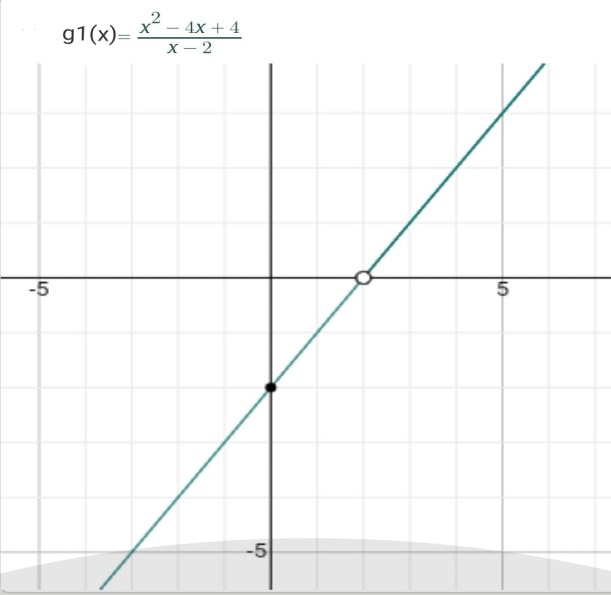
\includegraphics[width=2.77in,height=2.7in]{capitulos/outras_funcoes/media/image48.jpeg}
		\end{Center}
	\end{figure}

	c) \( R \left( x \right) =\frac{x-1}{x^{2}-x}\) \\ \(D= \{ x \in R/x \neq 0 e~x \neq 1 \}  \) \\ \( Im= \{ y \in R/y \neq 0 \} \)\\

	\( R1 \left( x \right) =\frac{1}{x}\) \\\(D= \{ x \in R/x \neq 0 \}  \) \\ \( Im= \{ y \in R/y \neq 0 \}  \)

	\begin{figure}[H]
		\begin{Center}
			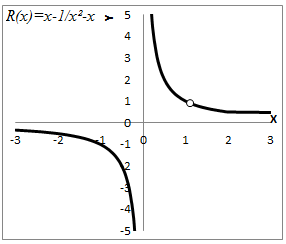
\includegraphics[width=2.98in,height=2.54in]{capitulos/outras_funcoes/media/image49.png}
		\end{Center}
	\end{figure}

	\begin{figure}[H]
		\begin{Center}
			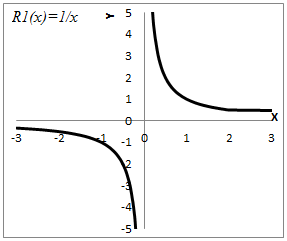
\includegraphics[width=2.99in,height=2.51in]{capitulos/outras_funcoes/media/image50.png}
		\end{Center}
	\end{figure}


	d)  \( H \left( x \right) =\frac{x^2+2x}{x}\) \\\(D= \{ x \in R/x \neq 0 \} \) \\ \( Im= \{ y \in R/y \neq 2 \}  \)\\

	\( H1 \left( x \right) =x+2\) \\\(D= \{ x \in R \}  \) \\ \( Im= \{ y \in R \}  \)

	\begin{figure}[H]
		\begin{Center}
			\includegraphics[width=2.76in,height=2.31in]{capitulos/outras_funcoes/media/image51.png}
		\end{Center}
	\end{figure}

	\begin{figure}[H]
		\begin{Center}
			\includegraphics[width=2.77in,height=2.31in]{capitulos/outras_funcoes/media/image52.png}
		\end{Center}
	\end{figure}

	e) \(q \left( x \right) =\frac{-x}{x- 1}\)\\ \(D= \{ x \in R/x \neq 1  \}  \) \\\( Im= \{ y \in R/y \neq -1  \}  \)\\

 	\( q1 \left( x \right) =\frac{-x^{2}-x}{x^2- 1}\)\\ \(D= \{ x \in R/~x \neq -1\text{ e x} \neq 1  \}  \)\\\( Im= \{ y \in R/y \neq -1\text{ e y} \neq -\frac{1}{2} \} \)

	\begin{figure}[H]
		\begin{Center}
			\includegraphics[width=2.94in,height=2.43in]{capitulos/outras_funcoes/media/image53.jpeg}
		\end{Center}
	\end{figure}

	\begin{figure}[H]
		\begin{Center}
			\includegraphics[width=2.94in,height=2.74in]{capitulos/outras_funcoes/media/image54.jpeg}
		\end{Center}
	\end{figure}

	f)  \( P \left( x \right) =\frac{x^2+4x+3}{x+3}\)\\\(D= \{ x \in R/ x \neq -3 \}  \) \\\( Im= \{ y \in R/y \neq -2 \}  \)\\

	\( P1 \left( x \right) =x+1\)\\\(D= \{ x \in R \}  \) \\ \( Im= \{ y \in R \} \)

	\begin{figure}[H]
		\begin{Center}
			\includegraphics[width=2.8in,height=2.31in]{capitulos/outras_funcoes/media/image55.png}
		\end{Center}
	\end{figure}

	~~

	\begin{figure}[H]
		\begin{Center}
			\includegraphics[width=2.77in,height=2.34in]{capitulos/outras_funcoes/media/image56.png}
		\end{Center}
	\end{figure}

	\ansitem{} a) Assíntota Horizontal: y\textit{=0}; Assíntota Vertical: \textit{x=1.}

	b) Assíntota Horizontal: y\textit{=1/2}; Assíntota Vertical: \textit{x=0.}

	c) Assíntota Horizontal: \textit{y=-1}; Assíntota Vertical: \textit{x=2.}
	\newpage
	\ansitem{} a) 

	\begin{figure}[H]
		\begin{Center}
			\includegraphics[width=2.96in,height=2.29in]{capitulos/outras_funcoes/media/image57.pdf}
		\end{Center}
	\end{figure}

	~~

	b)

	\begin{figure}[H]
		\begin{center}
			\includegraphics[width=0.45\textwidth]{capitulos/outras_funcoes/media/image58.pdf}
		\end{center}
	\end{figure}

	c)
	
	\begin{figure}[H]
		\begin{center}	
			\includegraphics[width=0.45\textwidth]{capitulos/outras_funcoes/media/image59.pdf}
		\end{center}
	\end{figure}

\end{respostas}

\begin{respostas}{4}

	\ansitem{} a)

	\begin{figure}[H]
		\begin{Center}
			\includegraphics[width=2.45in,height=1.85in]{capitulos/outras_funcoes/media/image60.pdf}
		\end{Center}
	\end{figure}

~~

	b)

	\begin{figure}[H]
		\begin{Center}
			\includegraphics[width=2.71in,height=2.25in]{capitulos/outras_funcoes/media/image61.pdf}
		\end{Center}
	\end{figure}

~~

	c)

	\begin{figure}[H]
		\begin{Center}
			\includegraphics[width=2.61in,height=2.17in]{capitulos/outras_funcoes/media/image62.pdf}
		\end{Center}
	\end{figure}

~~
	d)

	\begin{figure}[H]
		\begin{Center}
			\includegraphics[width=2.61in,height=2.17in]{capitulos/outras_funcoes/media/image63.pdf}
		\end{Center}
	\end{figure}

~~

	e)

	\begin{figure}[H]
		\begin{Center}
			\includegraphics[width=2.61in,height=2.17in]{capitulos/outras_funcoes/media/image64.pdf}
		\end{Center}
	\end{figure}

~~

	f)

	\begin{figure}[H]
		\begin{Center}
			\includegraphics[width=2.71in,height=2.25in]{capitulos/outras_funcoes/media/image65.pdf}
		\end{Center}
	\end{figure}

~~

	\ansitem{} a)~ \( D= \{ x \in R \}  \) \textbf{;  \( Im= \{ y \in R \}  \) }

	b)  \( D= \{ x \in R \}  \) \textbf{;  \( Im= \{ y \in R \}  \) }

	c)  \( D= \{ x \in R \}  \) \textbf{;  \( Im= \{ y \in R \}  \) }

	d)  \( D= \{ x \in R \}  \) \textbf{;  \( Im= \{ y \in R \}  \) }

	e)  \( D= \{ x \in R \}  \) \textbf{;  \( Im= \{ y \in R \}  \) }

	f)  \( D= \{ x \in R \}  \) \textbf{;  \( Im= \{ y \in R/y>-2,04 \}  \) }

	\ansitem{}  \( f \left( x \right) =\frac{3}{4}x^3-1 \) 

	\begin{figure}[H]
		\begin{Center}
			\includegraphics[width=2.71in,height=2.04in]{capitulos/outras_funcoes/media/image66.pdf}
		\end{Center}
	\end{figure}

~~

	\ansitem{}  \( g \left( x \right) =-\frac{3}{26}x^{3}-\frac{23}{26} \) 

	\begin{figure}[H]
		\begin{Center}
			\includegraphics[width=2.71in,height=2.08in]{capitulos/outras_funcoes/media/image67.pdf}
		\end{Center}
	\end{figure}

~~

	\ansitem{} \( h \left( x \right) =-\frac{2}{3}x^{3}+\frac{8}{3}x+1 \) 

	\begin{figure}[H]
		\begin{Center}
			\includegraphics[width=2.71in,height=2.08in]{capitulos/outras_funcoes/media/image68.pdf}
		\end{Center}
	\end{figure}

~~

	\ansitem{} \textit{q(x) = -x\textsuperscript{3}-4x\textsuperscript{2}+4.}

	\begin{figure}[H]
		\begin{Center}
			\includegraphics[width=2.71in,height=2.87in]{capitulos/outras_funcoes/media/image69.jpeg}
		\end{Center}
	\end{figure}

\end{respostas}

\begin{respostas}{5}
	\ansitem{} 
	\begin{multicols}{2}
		a) \( f \left( -1 \right) =-2 \)
		
		b) \( f \left( 0 \right) =1 \)

		c) \( f \left( -3 \right) =-2 \)
		
		d)  \( f \left( 1 \right) =1 \)
		
		e) \( f \left( 2 \right) =1 \)
				
	\end{multicols}

	\ansitem{} a)

	\begin{figure}[H]
		\begin{Center}
			\includegraphics[width=2.71in,height=2.2in]{capitulos/outras_funcoes/media/image70.png}
		\end{Center}
	\end{figure}

~~

	b)

	\begin{figure}[H]
		\begin{Center}
			\includegraphics[width=2.71in,height=2.2in]{capitulos/outras_funcoes/media/image71.png}
		\end{Center}
	\end{figure}

~~

	c)

	\begin{figure}[H]
		\begin{Center}
			\includegraphics[width=2.71in,height=2.2in]{capitulos/outras_funcoes/media/image72.pdf}
		\end{Center}
	\end{figure}

~~

	d)

	\begin{figure}[H]
		\begin{Center}
			\includegraphics[width=2.71in,height=2.2in]{capitulos/outras_funcoes/media/image73.pdf}
		\end{Center}
	\end{figure}

~~

	\ansitem{} a)

	\begin{figure}[H]
		\begin{Center}
			\includegraphics[width=2.2in,height=1.92in]{capitulos/outras_funcoes/media/image74.pdf}
		\end{Center}
	\end{figure}

~~

	b)

	\begin{figure}[H]
		\begin{Center}
			\includegraphics[width=2.71in,height=2.28in]{capitulos/outras_funcoes/media/image75.pdf}
		\end{Center}
	\end{figure}

~~

	\ansitem{} \( D= \{ x \in R \}  \) \\ \( Im= \{ y \in R/0<y<1 \} \)

	\begin{figure}[H]
		\begin{Center}
			\includegraphics[width=2.71in,height=2.05in]{capitulos/outras_funcoes/media/image76.pdf}
		\end{Center}
	\end{figure}

~~

	\ansitem{} \( D= \{ x \in R \}  \) \\ \( Im= \{ y \in R/0<y<1 \} \)

	\begin{figure}[H]
		\begin{Center}
			\includegraphics[width=2.71in,height=2.05in]{capitulos/outras_funcoes/media/image77.pdf}
		\end{Center}
	\end{figure}

~~

	\ansitem{} \( D= \{ x \in R \}  \) \\ $( Im= \{ y \in {R} / y=0 $ ou $ 1<y \leq 2 \}  $) 

	\begin{figure}[H]
		\begin{Center}
			\includegraphics[width=2.7in,height=2.32in]{capitulos/outras_funcoes/media/image78.pdf}
		\end{Center}
	\end{figure}
~~

	\ansitem{} \( D= \{ x \in R \} \) \\ \( Im= \{ y \in R/y \geq 0 \}  \)

	\begin{figure}[H]
		\begin{Center}
			\includegraphics[width=2.69in,height=2.01in]{capitulos/outras_funcoes/media/image79.pdf}
		\end{Center}
	\end{figure}
\end{respostas}
~~

\begin{respostas}{6}
	\ansitem{} a) A função é par\quad 

	b) A função é ímpar

	c) A função é par

	d) A função é ímpar

	e) A função é par

	f) A função é ímpar

	\ansitem{} A função é ímpar

	\ansitem{} A função é par

\end{respostas}

\begin{respostas}{7}

	\ansitem{} a) 7 

	b) Se  \( x+1 \geq 0; \vert x+1 \vert =x+1 \) 

	Se  \( x+1<0; \vert x+1 \vert =- \left( x+1 \right)  \) 

	c) 8

	d) Se  \( x-1 \geq 0; \vert x-1 \vert =x-1 \) 

	Se  \( x-1<0; \vert x-1 \vert =- \left( x-1 \right)  \) 

	e) Se  \( x \leq 2; \vert -x+2 \vert = \left( -x+2 \right)  \) 

	Se  \( x>2; \vert -x+2 \vert =- \left( -x+2 \right)  \) 

	f) Se  \( x \leq 5; \vert 5-x \vert = \left( 5-x \right)  \) 

	Se  \( x>5; \vert 5-x \vert =- \left( 5-x \right)  \) 

	\ansitem a) $( I= \{ x \in R/x<-1 $ ou $ x>1 \}  )$ 

	b) \( I= \{ x \in R/x \neq -1 \}  \) 

	c) \( I= \{ x \in R/-1<x<1 \}  \) 

	d) \( I= \{ x \in R /-1<x<3 \}  \) 

	e) \(  I= \{ x \in R /0<x<4 \}  \) 

	f) \( I= \{ x \in R /4<x<6 \}  \) 

	\ansitem{} a) 

	\begin{figure}[H]
		\begin{Center}
			\includegraphics[width=2.47in,height=0.57in]{capitulos/outras_funcoes/media/image80.png}
		\end{Center}
	\end{figure}

~~

	b)

	\begin{figure}[H]
		\begin{Center}
			\includegraphics[width=2.47in,height=0.62in]{capitulos/outras_funcoes/media/image81.png}
		\end{Center}
	\end{figure}

~~

	c)

	\begin{figure}[H]
		\begin{Center}
			\includegraphics[width=2.47in,height=0.48in]{capitulos/outras_funcoes/media/image82.png}
		\end{Center}
	\end{figure}

~~

	d)

	\begin{figure}[H]
		\begin{Center}
			\includegraphics[width=2.47in,height=0.54in]{capitulos/outras_funcoes/media/image83.png}
		\end{Center}
	\end{figure}

~~

	e)

	\begin{figure}[H]
		\begin{Center}
			\includegraphics[width=2.47in,height=0.65in]{capitulos/outras_funcoes/media/image84.png}
		\end{Center}
	\end{figure}

~~

	f)

	\begin{figure}[H]
		\begin{Center}
			\includegraphics[width=2.47in,height=0.88in]{capitulos/outras_funcoes/media/image85.png}
		\end{Center}
	\end{figure}

~~

	\ansitem{} a)  \( D= \{ x \in R \}  \) \textbf{; \( Im= \{ y \in R/y \geq 0 \}  \) }

	\begin{figure}[H]
		\begin{Center}
			\includegraphics[width=2.82in,height=2.09in]{capitulos/outras_funcoes/media/image86.pdf}
		\end{Center}
	\end{figure}

~~

	b)  \( D= \{ x \in R \}  \) \textbf{; \( Im= \{ y \in R/y \geq 0 \}  \) }

	\begin{figure}[H]
		\begin{Center}
			\includegraphics[width=2.71in,height=2.09in]{capitulos/outras_funcoes/media/image87.pdf}
		\end{Center}
	\end{figure}

~~

	c)  \( D= \{ x \in R \}  \) \textbf{; \( Im= \{ y \in R/y \geq 0 \}  \) }

	\begin{figure}[H]
		\begin{Center}
			\includegraphics[width=2.71in,height=2.09in]{capitulos/outras_funcoes/media/image88.pdf}
		\end{Center}
	\end{figure}

~~

	d)  \( D= \{ x \in R \}  \) \textbf{; \( Im= \{ y \in R/y \geq 0 \}  \) }

	\begin{figure}[H]
		\begin{Center}
			\includegraphics[width=2.71in,height=2.09in]{capitulos/outras_funcoes/media/image89.pdf}
		\end{Center}
	\end{figure}

	e)  \( D= \{ x \in R \}  \) \textbf{; \( Im= \{ y \in R/y \geq 0 \}  \) }

	\begin{figure}[H]
		\begin{Center}
			\includegraphics[width=2.71in,height=2.09in]{capitulos/outras_funcoes/media/image90.pdf}
		\end{Center}
	\end{figure}

	f)  \( D= \{ x \in R \}  \) \textbf{; \( Im= \{ y \in R/y \geq 2 \}  \) }

	\begin{figure}[H]
		\begin{Center}
			\includegraphics[width=2.74in,height=2.11in]{capitulos/outras_funcoes/media/image91.pdf}
		\end{Center}
	\end{figure}

	g)  \( D= \{ x \in R \}  \) \textbf{; \( Im= \{ y \in R/y \geq 4 \}  \) }

	\begin{figure}[H]
		\begin{Center}
			\includegraphics[width=2.71in,height=2.09in]{capitulos/outras_funcoes/media/image92.pdf}
		\end{Center}
	\end{figure}

~~

	h)  \( D= \{ x \in R \}  \) \textbf{; \( Im= \{ y \in R/y \geq 4 \}  \) }

	\begin{figure}[H]
		\begin{Center}
			\includegraphics[width=2.71in,height=2.09in]{capitulos/outras_funcoes/media/image93.pdf}
		\end{Center}
	\end{figure}

~~

	i)  \( D= \{ x \in R \}  \) \textbf{; \( Im= \{ y \in R/y \geq -1 \}  \) }

	\begin{figure}[H]
		\begin{Center}
			\includegraphics[width=2.71in,height=2.09in]{capitulos/outras_funcoes/media/image94.pdf}
		\end{Center}
	\end{figure}

~~

	\ansitem{} a)


	\begin{figure}[H]
		\begin{Center}
			\includegraphics[width=2.6in,height=2.15in]{capitulos/outras_funcoes/media/image95.pdf}
		\end{Center}
	\end{figure}

~~

	b)

	\begin{figure}[H]
		\begin{Center}
			\includegraphics[width=2.6in,height=2.15in]{capitulos/outras_funcoes/media/image96.pdf}
		\end{Center}
	\end{figure}

~~

	c)

	\begin{figure}[H]
		\begin{Center}
			\includegraphics[width=2.6in,height=2.15in]{capitulos/outras_funcoes/media/image97.pdf}
		\end{Center}
	\end{figure}

~~

	d)

	\begin{figure}[H]
		\begin{Center}
			\includegraphics[width=2.6in,height=2.15in]{capitulos/outras_funcoes/media/image98.pdf}
		\end{Center}
	\end{figure}

~~

	e)

	\begin{figure}[H]
		\begin{Center}
			\includegraphics[width=2.6in,height=2.15in]{capitulos/outras_funcoes/media/image99.pdf}
		\end{Center}
	\end{figure}

~~
	f)

	\begin{figure}[H]
		\begin{Center}
			\includegraphics[width=2.6in,height=2.15in]{capitulos/outras_funcoes/media/image100.pdf}
		\end{Center}
	\end{figure}

\end{respostas}

